\pagebreak
\thispagestyle{empty}
\movetoevenpage
\begin{figure}
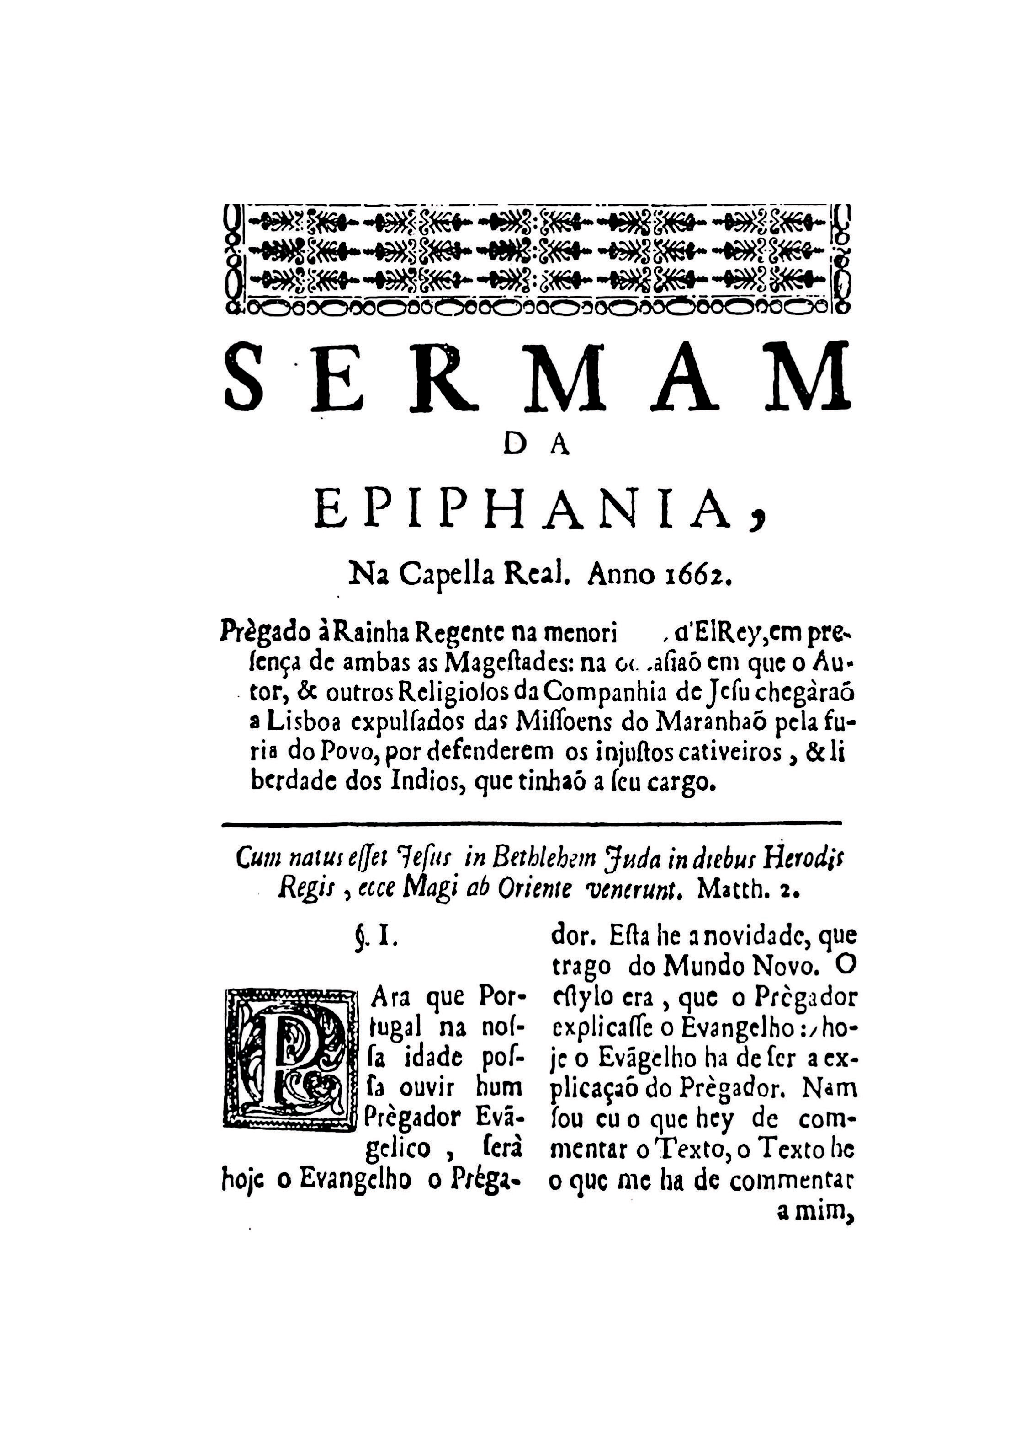
\includegraphics[width=\textwidth]{./imgs/epifania.pdf}  
\end{figure}

\chapter{Sermão da Epifania}


\begin{quotation}
\noindent{}Na Capela Real. Ano de 1662.\\
Pregado à Rainha Regente na menoridade de el Rei, em presença
de ambas as Majestades: na ocasião em que o Autor e outros
Religiosos da Companhia de Jesus chegaram a Lisboa expulsados
das Missões do Maranhão pela fúria do Povo, por defenderem
os injustos cativeiros, e liberdade dos Índios que tinham a
seu cargo.
\end{quotation}


\epigraph{\emph{Cum natus esset Jesus in Bethlehem Juda in diebus Herodis regis,
ecce Magi ab oriente venerunt.}}{Mt, 2.}

\section{I}

\noindent{}Para que Portugal na nossa idade possa ouvir um pregador evangélico,
será hoje, o Evangelho o pregador. Esta é a novidade que trago do Mundo
Novo. O estilo era que o pregador explicasse o Evangelho: hoje o
Evangelho há de ser a explicação do pregador. Não sou eu o que hei de
comentar o texto: o texto é o que me há de comentar a mim. Nenhuma
palavra direi que não seja sua, porque nenhuma cláusula tem que não seja
minha. Eu repetirei as suas vozes, ele bradará os meus silêncios. Praza
a Deus que os ouçam os homens na terra, para que não cheguem a ser
ouvidos no céu.

Havendo, porém, de pregar o Evangelho, e com tão novas circunstâncias
como os que promete o exórdio, nem por isso cuide alguém que o pregador
e o sermão há de faltar ao mistério. Antes, pode bem ser que rara vez ou
nunca se pregasse neste lugar a matéria própria deste dia e desta
solenidade senão hoje o mistério próprio deste dia é a vocação da
gentilidade à fé. Até agora celebrou a Igreja o nascimento de Cristo;
hoje celebra o nascimento da Cristandade. \emph{Cum natus esset Jesus in
Bethlehem Juda}: este foi o nascimento de
Cristo, que já passou: \emph{Ecce Magi ab Oriente venerun}:
 este é o nascimento da Cristandade, que hoje se
celebra. Nasceu hoje a Cristandade, porque os três reis que neste dia
vieram adorar a Cristo foram os primeiros que o reconheceram por Senhor,
e por isso lhe tributaram ouro; os primeiros que o reconheceram por
Deus, e por isso lhe consagraram incenso, os primeiros que o
reconheceram por homem em carne mortal, e por isso lhe ofereceram mirra.
Vieram gentios, e tornaram fiéis, vieram idólatras, e tornaram cristãos;
e esta é a nova glória da Igreja, que ela hoje celebra, e o Evangelho,
nosso pregador, refere. Demos"-lhe atenção.

\section{II}

\emph{Cum natus esset Jesus in Bethlehem Juda in diebus Herodis regis,
ecce Magi ab Oriente venerunt.} Estas são as primeiras palavras do
Evangelho, e logo nelas parece que repugna o mesmo Evangelho a ser meu
intérprete, porque a sua história e o seu mistério é da Índia Oriental:
\emph{Ab oriente venerunt}, e o meu caso é das Ocidentais. Se apelo
para os reis e para o sentido místico, também está contra mim, porque
totalmente exclui a América, que é a parte do mundo donde eu venho.
Santo Agostinho, S.\,Leão papa, S.\,Bernardo, Santo Anselmo, e quase todos
os Padres reparam, por diversos modos, em que os reis que vieram adorar
a Cristo fossem três, e a limitação deste mesmo número é para mim, ou
contra mim, o maior reparo. Os profetas tinham dito que todos os reis e
todas as gentes haviam de vir adorar e reconhecer a Cristo:
\emph{Adorabunt eum omnes reges terrae, omnes gentes serviente ei}:
\emph{Omnes gentes quascumquefecisti veniente, et
adorabunt te, corai Dominet}. Pois, se todas as
gentes e todos os reis do mundo haviam de vir adorar a Cristo, por que
vieram somente três? Por isso mesmo, respondem o Venerável Beda e
Ruperto Abade. Foram três, e nem mais nem menos que três, os Reis que
vieram adorar a Cristo, porque neles se
representavam todas as partes do mundo, que também são três: Ásia,
África e Europa: \emph{Tres reges, tres partes mundi significant: Asiam,
Africam, et Europam,} diz Beda. E Ruperto, com a mesma distinção:
\emph{Magi tribus partibus orbis, Asiae, Europae, atque Africae, pidei,
atque adorationis exemplar existere meruerunt.} Isto é o que dizem estes
grandes autores, como intérpretes do Evangelho; mas o mesmo Evangelho,
para ser meu intérprete, ainda há de dizer mais. Dizem que os três reis
significavam a Ásia, a África e a Europa, e onde lhes ficou a América? A
América não é, também, parte do mundo, e a maior parte? Se me disserem
que não apareceu no presépio, porque tardou e veio muitos séculos
depois, também as outras tardaram; antes, ela tardou menos, porque se
converteu e adorou a Cristo mais depressa e mais sem repugnância que
todas. Pois, se cada um das outras partes do mundo teve o seu rei que as
apresentasse a Cristo, por que lhe há de faltar pobre América? Há de ter
rei que receba e se enriqueça com os seus tributos, e não há de ter rei
que com eles ou sem eles a leve aos pés de Cristo? Sei eu: e não o
pode negar a minha dor que se a primeira, segunda, e a terceira parte do
mundo tiveram reis, também o teve a quarta, e enquanto lhe não faltou o
quarto. Mas vamos ao Evangelho, e conciliemos com ele
esta exposição dos Padres.

\emph{Ecce Magi ab oriente venerunt.} Diz o Evangelista que os reis do
Oriente vieram a adorar a Cristo, e nesta mesma limitação, com que diz
que vieram nomeadamente os do Oriente, e não outros, se reforça mais a
dúvida, porque assim no Testamento Velho, como no Novo, está expresso
que não só haviam de vir a Cristo os gentios do Oriente, senão também os
do Ocidente. No testamento Velho, Isaías, falando com a Igreja: \emph{Ab
oriente adducam semen tuum, et ab occidente congregabo te};
e no Testamento Novo a profecia e oráculo de Cristo:
\emph{Dico vobis, quod multi ab oriente et occidente venient.} Pois,
se não só haviam de vir a Cristo os reis e gentes do Oriente, senão
também as do Ocidente, como diz nomeadamente o evangelista que os que
vieram eram todos do Oriente, ou como vieram só os do Oriente, e os do
Ocidente não? A tudo satisfez o mesmo evangelista, e na simples narração
da história concordou admiravelmente o seu texto com o dos profetas. Que
diz o evangelista? \emph{Cum natus esset Jesus in diebus Herodis regis,
ecce Magi ab oriente venerunt.} Diz que nos dias de Herodes, sendo
nascido Cristo, o vieram adorar os Reis do Oriente: e nestas mesmas
circunstâncias do tempo, do lugar e das pessoas, como que limitou a
primeira vocação da gentilidade, mostrou que não havia de ser só uma,
senão duas, como estava profetizado. A primeira vocação da gentilidade
foi nos dias de Herodes: \emph{In diebus Herodis regis}; a segunda
quase em nossos dias. A primeira foi quando Cristo nasceu: \emph{Cum
natus esset Jesus}; a segunda quando já se contavam mil e quinhentos
anos do nascimento de Cristo. A primeira foi por meio dos reis do
Oriente: \emph{Ecce Magi ab oriente venerunt}; a segunda por meio dos
reis do Ocidente, e dos mais ocidentais de todos, que são os de
Portugal.

Para melhor inteligência destas duas vocações, ou destas duas epifanias,
havemos de supor que neste mesmo mundo em diferentes tempos houve dois
mundos: O Mundo Velho, que conheceram os antigos, e o Mundo Novo, que
eles e o mesmo mundo não conheceu, até que os portugueses o descobriram.
O mundo Velho compunha"-se de três partes: Ásia, África e Europa, mas de
tal maneira que, entrando neste primeiro composto toda a Europa, a Ásia
e a África não entravam inteiras, senão partidas, e por um só lado, a
África com toda a parte que abraça o Mar Mediterrâneo, e a Ásia com a
parte a que se estende o Mar Eritreu. O Mundo Novo, muito maior que o
Velho, também se compõe de três partes: Ásia, África e América, mas de
tal maneira também, que entrando neste segundo composto toda a América,
a Ásia e a África, só entram nele partidas, e com os outros dois lados,
tanto mais vastos e tanto mais dilatados, quanto o mar Oceano que os
rodeia excede ao Mediterrâneo e Eritreu. E como os autores antigos só
conheceram o Mundo Velho, e não tiveram nem podiam ter conhecimento do
novo, por isso Beda e Ruperto disseram com muita propriedade que os três
Reis do Oriente representavam as três partes do mundo: Ásia, África e
Europa. Contudo, S.\,Bernardo, que foi contemporâneo de Ruperto,
combinando o nosso Evangelho com as outras Escrituras, conheceu com seu
grande espírito, ou, quando menos, arguiu com seu grande engenho que,
assim como houve três reis do Oriente que levaram as gentilidades a
Cristo, assim havia de haver outros três reis do Ocidente que as
trouxessem à mesma fé: \emph{Vide autem neforte ipsi sint et tres Magi
venientes iam non ab Oriente sed etiam ab Occidentel}.
Quem fossem ou quem houvessem de ser estes três reis do Ocidente, que S.\,Bernardo anteviu, não o disse, nem o pôde dizer o mesmo santo, posto que
tão devoto de Portugal, e tão familiar amigo do nosso primeiro rei. Mas
o tempo, que é o mais claro intérprete dos futuros, nos ensinou dali a
quatrocentos anos que estes felicíssimos reis foram el"-rei D.\,João, o
Segundo, el"-rei D.\,Manuel, e el rei D.\,João, o Terceiro, porque o
primeiro começou, o segundo prosseguiu, e o terceiro aperfeiçoou o
descobrimento das nossas conquistas, e todos três trouxeram ao
conhecimento de Cristo aquelas novas gentilidades, como os três Magos as
antigas. Os Magos levando a luz da fé do Oriente para o Ocidente, eles
do Ocidente para o Oriente;
os Magos apresentando a Cristo a Ásia, África e Europa, e eles a Ásia,
África e América: Os Magos estendendo os raios da sua estrela por todo o
Mundo Velho, até às gargantas do Mediterrâneo, e eles alumiando com o
novo sol a todo o Mundo Novo até às balizas do Oceano.

Uma das coisas mais notáveis que Deus revelou e prometeu antigamente foi
que ainda havia de criar um novo céu, e uma nova terra. Assim o disse
por boca do profeta Isaías: \emph{Ecce ego creo caelos novos, et terram
novam}. É certo que o céu e a terra foram criados no
princípio do mundo: \emph{In principio creavit Deus caelum et terram},
e também é certo, entre todos os teólogos
e filósofos, que depois daquela primeira criação, Deus não criou nem
cria substância alguma material e corpórea porque somente cria de novo
as almas, que são espirituais. Logo, que terra nova, e que céus novos
são estes, que Deus tanto tempo antes prometeu que havia de criar?
Outros o entendem doutra maneira, não sei se muito conforme à letra. Eu,
seguindo o que ela simplesmente soa e significa, digo que esta nova
terra e estes novos céus são a terra e os céus do Mundo Novo, descoberto
pelos Portugueses. Não é verdade que, quando os nossos argonautas
começaram e prosseguiram as suas primeiras navegações, iam juntamente
descobrindo novas terras, novos mares, novos climas, novos céus, novas
estrelas? Pois esta é a terra nova e esses são os céus novos que Deus
tinha prometido, que havia de criar, não porque não estivessem já
criados desde o princípio do mundo, mas porque era este Mundo Novo, tão
oculto e ignorado dentro do mesmo mundo, que quando de repente se
descobriu e apareceu, foi como se então começara a ser e Deus o criara
de novo. E porque o fim deste descobrimento, ou desta nova criação, era
a Igreja, também nova, que Deus pretendia fundar no mesmo Mundo Novo,
acrescentou logo pelo mesmo profeta e, pelos mesmos termos, que também
havia de criar uma nova Jerusalém, isto é, uma nova Igreja, na qual
muito se agradasse: \emph{Quia ecce creo Jerusalém exultationem, et
populum ejus gaudium}.

Não tenho menos autor deste pensamento que o evangelista dos segredos de
Deus, S.\,João, no seu Apocalipse: \emph{Etvidi caelum novum etterram
novam. Primum enim caelum, et prima terra abiit, et mare jam non est. Et
vidi civitatem Jerusalém novam descendentem de caelo}.
Primeiramente, diz S.\,João que viu um céu novo e uma terra
nova: \emph{Vidi caelum novum et terram novam.} Esta é a terra nova e o
céu novo que Deus tinha prometido por Isaías. Logo, acrescenta o mesmo
evangelista, como comentador do profeta, que à vista deste céu novo e
desta terra nova, o céu e a terra antiga desapareceram, e que o mar já
não era: \emph{Primum} enim \emph{caelum, et prima terra abiit, et mare
iam non est}, e assim aconteceu no descobrimento do Mundo Novo.
Desapareceu a terra antiga, porque a terra dali por diante já não era a
que tinha sido, senão outra muito maior, muito mais estendida e dilatada
em novas costas, em novos cabos, em novas ilhas, em novas regiões, em
novas gentes, em novos animais, em novas plantas. Da mesma maneira o céu
também começou a ser outro. Outros astros, outras figuras celestes,
outras alturas, outras declinações, outros aspectos, outras influencias,
outras luzes, outras sombras, e tantas outras coisas todas outras.
Sobretudo o mar, que fora, já não é: \emph{Et mare jam non est},
porque até então o que se conhecia com nome de mar, e nas mesmas
Escrituras se chama \emph{mare magnum,} era o Mediterrâneo; mas, depois
que se descobriu o Mundo Novo, logo se conheceu também que não era
aquele o mar, senão braço dele, e o mesmo nome, que injustamente tinha
usurpado, se passou sem controvérsia ao oceano, que é só o que por sua
imensa grandeza absolutamente, e sem outro sobrenome, se chama mar. E
porque toda esta novidade do novo céu, da nova terra e do novo mar, se
ordenava à fundação de outra nova Igreja, esta foi a que logo viu o
mesmo evangelista, com nome também de nova: \emph{Et vidi civitatem
Jerusalem novam descendentem de caelo.} Finalmente, para que ninguém
duvidasse de toda esta explicação, conclui que a mesma Igreja nova que
vira se havia de compor de nações e reis gentios, que nela receberiam a
luz da fé, e sujeitariam suas coroas ao império de Cristo: \emph{Et
ambulabunt gentes in lumine ejus ei reges terrae afferent gloriam suam
ei honorem in illam}. Que é tudo o que temos visto
no descobrimento do Mundo Novo, ou nesta nova criação dele: \emph{Ecce
creo caelos novos ei íerram novam.}

Houve porém nesta segunda e nova criação do mundo, uma grande diferença
da primeira, e de nova e singular glória para a nossa nação. Porque,
havendo Deus criado o mundo na primeira criação por si só, e sem ajuda
ou concurso de causas segundas, nesta segunda criação tomou por
instrumento dela os portugueses, quase pela mesma ordem e com as mesmas
circunstâncias, com que no princípio tinha criado o mundo.
Quando Deus criou o mundo, diz o sagrado texto que a terra não se via
porque estava escondida debaixo do elemento da água, e tudo escuro e
coberto de trevas: \emph{Terra autem erat invisibilis}, como lêem os
Setenta \emph{et tenebrae erani super faciem abyssi}. Então dividiu Deus as águas, e apareceu a terra; criou a luz e cessaram as trevas: \emph{Divisit aquas;
facta est lux; appareat Arida}. Este foi o modo da
primeira criação do mundo. E quem não vê que o mesmo observou Deus na
segunda, por meio
dos portugueses? Estava todo o Novo Mundo em trevas e às escuras, porque
não era conhecido. Tudo o que ali havia, sendo tanto, era como se não
fosse nada, porque assim se cuidava e tinha por fábula. \emph{Terra
autem erat vanitas ei nihil,} como diz o texto hebreu.
O que encobria a terra era o elemento da água, porque a
imensidade do Oceano, que estava em meio, se julgava por insuperável,
como a julgaram todos os antigos, e entre eles Santo Agostinho.
Atreveu"-se, finalmente, a ousadia e zelo dos portugueses a desfazer este
encanto e vencer este impossível. Começaram a dividir as águas, nunca
dantes cortadas, com as venturosas proas dos seus primeiros lenhos:
foram aparecendo e surgindo de uma e outra parte, e como nascendo de
novo, as terras, as gentes, o mundo que as mesmas águas encobriam, e não
só acabaram então no mundo antigo as trevas desta ignorância, mas muito
mais no novo e descoberto as trevas da infidelidade, porque amanheceu
nelas a luz do Evangelho e o conhecimento de Cri sto, o qual era o que
guiava e levava os portugueses, e neles, e com eles navegava. Tudo
estava vendo o mesmo profeta Isaías deste descobrimento, quando, falando
com aquela nova igreja, pelos mesmos termos da primeira criação do
mundo, lhe disse: \emph{Quia ecce tenebrae operient terram, ei caligo
populos; super te autem orietur Dominus, et gloria ejus in te videbitur.
Et ambulabuní gentes in lumine tuo, ei reges in splendore ortus
tui}.

\section{III}

Isto é o que fizeram os primeiros argonautas de Portugal, nas suas tão
bem afortunadas conquistas do Novo Mundo, e por isso bem afortunadas.
Este é o fim para que Deus, entre todas as nações, escolheu a nossa com
o ilustre nome de pura na fé, e amada pela piedade. Estas são as gentes
estranhas e remotas, aonde nos prometeu que havíamos de levar seu
Santíssimo Nome. Este é o império seu, que por nós quis amplificar e em
nós estabelecer. E esta é, foi, e será sempre a maior e melhor glória do
valor, do zelo, da religião e cristandade portuguesa. Mas quem dissera
ou imaginam que os tempos e os costumes se haviam de trocar, e fazer tal
mudança, que esta mesma glória nossa se visse entre nós eclipsada, e por
nós escurecida? Não quisera passar a matéria tão triste, e tão indigna:
que por isso a fui dilatando tanto, como quem rodeia e retarda os
passos, por não chegar aonde muito repugna. Mas nem a força da
presente ocasião mo permite, nem a verdade de um discurso, que prometeu
ser evangélico, o consente. Quem imaginara, torno a dizer, que aquela
glória tão heroicamente adquirida nas três partes do mundo, e tão
celebrada e esclarecida em todas as quatro, se havia de escurecer e
profanar em um rincão ou arrabalde da América?

Levantou o demônio este fumo ou assoprou este incêndio entre as palhas
de quatro choupanas, que com nome da cidade de Belém puderam ser pátria
do anticristo. E verdadeiramente que, se as Escritoras nos não ensinaram
que este monstro há de sair de outra terra e de outra nação, já
pudéramos cuidar que era nascido. Treme, e tem horror a língua de
pronunciar o que viram os olhos, mas, sendo o caso tão feio, tão
horrendo, tão atroz, e tão sacnlego que se não pode dizer, é tão público
e tão notório que se não deve calar. Ouçam, pois, os excessos de tão
nova e tão estranha maldade os que só lhe podem pôr o remédio; e se eles,
o que se não crê, faltarem à sua obrigação, não é justo, nem Deus o
permitirá, que eu falte à minha. O ofício que tive naquele lugar, e o
que tenho neste, posto que indigno de ambos, são os que, com dobrado
vínculo da consciência, me obrigam a romper o silencio, até agora
observado ou suprimido, esperando que a mesma causa, por ser de Cristo,
falasse e perorasse por si, e não por ela. Assim o fizeram em
semelhantes, e ainda menores casos, os Atanásios, os Basílios, os
Nazianzenos, os Crisóstomos, os Hilários, e todos aqueles grandes Padres
e mestres da Igreja, cujas ações, como inspiradas e aprovadas por Deus,
não só devemos venerar e imitar como exemplos, mas obedecer e seguir
como preceitos. Falarei, pois, com a clareza e publicidade com que eles
falaram, e provarei e farei certo o que disser, como eles o fizeram,
porque, sendo perseguidos e desterrados, eles eram o corpo do delito que
acusavam, e eles mesmos a prova. Assim permitiu a divina Providência que
eu em tal forma, e as pessoas reverendas de meus companheiros, viéssemos
remetidos aos olhos desta corte, para que ela visse e não duvidasse de
crer o que doutro modo pareceria incrível.

Quem havia de crer que em uma colônia chamada de portugueses se viesse a
Igreja sem obediência, as censuras sem temor, o sacerdócio sem respeito,
e as pessoas e lugares sagrados sem imunidade? Quem havia de crer que
houvessem de arrancar violentamente de seus claustros aos religiosos, e
levá"-los presos entre beleguins e espadas nuas pelas ruas públicas, e
tê"-los aferrolhados, e com guardas, até os desterrarem? Quem havia de
crer que com a mesma violência e afronta lançassem de suas cristandades
aos pregadores do Evangelho, com escândalo nunca imaginado dos antigos
cristãos, sem pejo dos novamente convertidos, e à vista dos gentios
atônitos e pasmados? Quem havia de crer que até aos mesmos párocos não
perdoassem, e que
chegassem aos despojos de suas igrejas, com interdito total do culto
divino e uso de seus ministérios: as igrejas ermas, os batistérios
fechados, os sacrários sem sacramento enfim, o mesmo Cristo privado de
seus altares, e Deus de seus sacrifícios? Isto é o que lá se viu então:
e que será hoje o que se vê, e o que se não vê. Não falo dos autores e
executores destes sacrilégios, tantas vezes, e por tantos títulos
excomungados, porque lá lhes ficam papas que os absolvam. Mas que será
dos pobres e miseráveis índios, que são a presa e os despojos de toda
esta guerra? Que será dos cristãos? Que será dos catecúmenos? Que será
dos gentios? Que será dos pais, das mulheres, dos filhos, e de todo o
sexo e idade? Os vivos e sãos sem doutrina, os enfermos sem sacramentos,
os monos sem sufrágios nem sepultura, e tanto gênero de almas em extrema
necessidade sem nenhum remédio? Os pastores, parte presos e desterrados,
parte metidos pelas brenhas; os rebanhos despedaçados; as ovelhas, ou
roubadas, ou perdidas; os lobos famintos, fartos agora de sangue, sem
resistência; a liberdade por mil modos trocada em servidão e cativeiro;
e só a cobiça, a tirania, e sensualidade, e o inferno contentes. E que a
tudo isto se atrevessem e atrevam homens com nomes de portugueses, e em
tempo de rei português?

Grandes desconcertos se lêem no mesmo capítulo do nosso Evangelho, mas
de todos acho eu a escusa nas primeiras palavras dele: \emph{In diebus
Herodis regis.} Se sucederam semelhantes escândalos nos dias de el"-rei
Herodes, o tempo os desculpava ou culpava menos; mas nos dias daquele
monarca, que com o nome e com a coroa herdou o zelo, a fé, a religião, a
piedade do grande Afonso I? Oh! que paralelo tão indigno do nome
português se pudera formar na comparação de tempo a tempo! Naquele tempo
andavam os portugueses sempre com as armas às costas contra os inimigos
da fé, hoje tomam as armas contra os pregadores da fé; então
conquistavam e escalavam cidades para Deus, hoje conquistam e escalam as
casas de Deus; então lançavam os caciques fora das mesquitas, hoje
lançam os sacerdotes fora das igrejas; então consagravam os lugares
profanos em casas de oração, hoje fazem das casas de oração lugares
profanos; então, finalmente, eram defensores e pregadores do nome
cristão, hoje são perseguidores e destruidores, e opróbrio e infâmia do
mesmo nome.

E para que até a corte e assento dos reis, que lhe sucederam, não
ficasse deste paralelo, então saíam pela barra de Lisboa as nossas naus
carregadas de pregadores, que voluntariamente se desterravam da pátria
para pregar nas conquistas a lei de Cristo, hoje entram pela mesma
barra, trazendo desterrados violentamente os mesmos pregadores, só
porque defendem nas conquistas a lei de Cristo. Não se envergonhe já a
barra de Argel de que entrem por elas sacerdotes de Cristo cativos e
presos, pois o mesmo se viu em nossos dias na barra de Lisboa. Oh! que
bem empregado prodígio fora neste caso, se, fugindo daquela barra o mar,
e voltando atrás o Tejo, lhe pudéssemos dizer, como ao rio e ao mar da
terra que então começava a ser santa: \emph{Quid est tibi, mare,
quodfugisti? Ei tu, Jordanis, quia conversus es retrorsum}?
Gloriava"-se o Tejo quando nas suas ribeiras se fabricavam e pelas suas
correntes saíam as armadas conquistadoras do império de Cristo;
gloriava"-se, digo, de ser ele aquele famoso rio de quem cantavam os
versos de Davi: \emph{Dominabitur a mari usque ad mare, ai a flumine
usque ad terminas orbis terra rum}; mas hoje, envergonhado
de tão afrontosa mudança, devera tornar atrás, e ir"-se esconder nas
grutas do seu nascimento, se não é que de corrido corre ao mar para se
afogar e sepultar no mais profundo dele.
Desengane"-se, porém, Lisboa que o mesmo mar lhe está lançando em rosto o
sofrimento de tamanho escândalo, e que as ondas, com que escumando de
ira batem as suas praias, são brados com que lhe está dizendo as mesmas
injúrias que antigamente a Sidônia: \emph{Erubesce, Sidon, ah mare}.

E não cuide alguém que estas vozes de tão justo sentimento nascem de
estranhar eu ou me admirar de que os pregadores de Cristo e o mesmo
Cristo seja perseguido, porque esta é a estrela em que o mesmo Senhor
nasceu: \emph{Cum natus esset Jesus in Bethlehem Juda in diebus Herodis
regis.} Ainda Cristo não tinha quinze dias de nascido, quando já Herodes
tinha poucos menos de perseguidor seu, para que a perseguição e o
perseguido nascessem juntos. E não só nasceu Cristo com estrela de
perseguido em Belém, senão em todas as partes do mundo, porque em todas
teve logo seu Herodes que o perseguisse. Vou supondo, como
verdadeiramente é, que Cristo não só nasceu em Belém, mas que nasceu e
nasce em outras muitas partes, como há de nascer em todas. Por isso o
profeta Malaquias, muito discretamente, comparou o nascimento de Cristo
ao nascimento do sol: \emph{Orietur vobis Sol justitiae}. O
sol vai nascendo sucessivamente a todo o mundo, e, ainda que a umas
terras nasça mais cedo, a outras mais tarde, para cada terra tem seu
nascimento. Assim também Cristo, verdadeiro sol. A primeira vez nasceu
em Belém, depois foi nascendo sucessivamente por todo o mundo, conforme
o foram pregando os apóstolos e seus sucessores: a umas terras nasceu
mais depressa, a outras mais devagar, a umas muito antes, a outras muito
depois, mas para todas teve seu nascimento. É a energia com que falou o
anjo aos pastares: \emph{Natus est vobis hodie Salvator}: % (Lc. 2,11)
Nasceu hoje para vós o Salvador, como se dissera: Hoje nasceu
para vós; os outros, também, terão seu dia em que há de nascer para
eles. Assim havia de ser, e assim foi, e assim tem nascido Cristo em
diferentes tempos em tão diversas partes do mundo, mas em nenhum tempo,
e em nenhuma parte nasceu onde logo não tivesse um Herodes que o
perseguisse.

Viu S.\,João no Apocalipse aquela mulher celestial vestida de sol, a qual
estava em vésperas do parto, e diz que logo apareceu diante dela um
dragão feroz e armado, o qual estava aguardando que saísse à luz o filho
para o tragar e comer: \emph{Et draco stetit ante mulierem, quae
eratparitura: utcumpeperisset,fihium ejus devoraret}. Que
mulher, que filho, e que dragão é este? A mulher foi a Virgem Maria, e é
a Igreja. O Filho foi e é Cristo, que assim como a primeira vez nasceu
da Virgem Santíssima, assim nasceu e nasce muitas vezes da Igreja, por
meio da fé e pregação de seus ministros em diversas partes do mundo. E o
dragão que apareceu com a boca aberta para o tragar, tanto que nascesse,
é cada um dos tiranos que logo mesmo Crista tem armados contra si, tanto
que nasce, e onde quer que nasce. De maneira que não há nascimento de
Cristo sem o seu perseguidor ou o seu Herodes. Nasceu Cristo em Roma,
pela pregação de S.\,Pedro, e logo se levantou um Herodes, que foi o
imperador Nero, o qual crucificou ao mesmos. Pedro. Nasceu Cristo em
Espanha, pela pregação de S.\,Tiago, e logo se levantou outro Herodes,
que foi el"-rei Agripa, o qual degolou ao mesmo S.\,Tiago.
Nasceu Cristo em Etiópia, pela pregação de S.\,Mateus, e logo se levantou
outro Herodes, que foi el"-rei Hirtaco, o qual tirou, também, a vida ao
mesmo S.\,Mateus, e, estando sacrificando o corpo de Cristo, o fez vítima
de Cristo, E para que dos exemplos do Mundo Velho passemos aos do Novo,
nasceu Cristo no Japão, pela pregação e milagres de S.\,Francisco Xavier,
e lago se levantaram, não um, senão muitos Herodes, que foram os
Nabunangas e Taicozamas, os quais tanta sangue derramaram, e ainda
derramam, dos filhos e sucessores do mesmo Xavier. Finalmente, nasceu
Cristo na conquista do Maranhão, que foi a última de todas as nossas, e
para que lhe não faltassem naquele Belém e fora dele os seus Herodes, se
levantaram agora e declaram contra Cristo em si mesmo, e em seus
pregadores, os que tão ímpia e barbaramente, não sendo bárbaros, o
perseguem. Assim que não é coisa nova, nem matéria digna de admiração,
que Cristo e os pregadores de sua fé sejam perseguidos.

O que, porém, excede toda o espanto, e se não pode ouvir sem horror e
assombro, é que as perseguidores de Cristo e seus pregadores neste casa
não sejam os infiéis e gentios, senão os cristãos. Se os gentios
indômitos, se as tapuias bárbaros e feras daquelas brenhas se armaram
medonhamente contra as que lhes vão pregar a fé, se os cobriram de
setas, se os fizeram em pedaços, se lhes arrancaram as entranhas
palpitantes, e as lançaram no fogo, e as comeram, isso é o que eles já
têm feito outras vezes, e a que lá vão buscar os que pelas salvar deixam
tudo; mas que a estes homens, com o caráter de ministras de Cristo, os
persigam gentilicamente os cristãos, quando essas mesmas feras se lhes
humanam, quando esses mesmos bárbaros se lhes rendem, quando esses
mesmos gentios os reverenciam e adoram, este é o maior extrema de
perseguição, e a perseguição, mais feia e afrontosa que nunca padeceu a
Igreja. Nas perseguições dos Neros e Dioclecianos os gentios perseguiam
os mártires, e as cristãos as adoravam; mas nesta perseguição nova e
inaudita, os cristãos são os que perseguem os pregadores, e os gentios
as que os adoram. Só na perseguição de Herades e na paciência de Cristo
se acham juntos estes extremos. No Evangelho temos a Cristo hoje
perseguido, e hoje adorada, mas de quem adorado, e de quem perseguido?
Adorado dos gentios, e perseguida dos cristãos, adorado das Magos, que
eram gentios, e perseguido de Herodes e de toda a Jerusalém, que eram os
cristãos daquele tempo.

Ninguém repare em eu lhes chamar cristãos, parque há cristãos de fé e
cristãos de esperança. Os filhos da Igreja somos cristãos de fé, parque
cremos que Cristo já veio; os filhos da sinagoga eram cristãos de
esperança, parque criam e esperavam que Cristo havia de vir. E que
homens que criam em Cristo, e esperavam por Cristo, e eram da mesma
nação e do mesmo sangue de Cristo, persigam tão barbaramente a Cristo, e
que no mesmo tempo, para maior escândalo da fé e da natureza, os Magos o
busquem, os gentios o creiam, os idólatras o adorem? Bendito sejais,
Senhor, que tal contradição quisestes padecer, e bendito mil vezes pela
parte que vos dignastes comunicar dela aos que tão indignamente vos
servem: não debalde nos honrastes com o nome de Companhia de Jesus,
obrigando"-nas a vos fazer companhia no que padecestes nascido debaixo do
mesmo nome: \emph{Cum natus esset Jesus in Bethlehem Juda.} Vós em Belém
de Judá, para que os vossos perseguidores fossem da vossa mesma nação,
nós em Belém, não de Judá, para que os nossos fossem, também, da nossa;
vós na mesma terra, e no mesma tempo perseguida de Herodes e adorado dos
Magos, e nós também por mercê vossa, no mesmo tempo e na mesma terra
perseguidos dos cristãos, e pouca menos que adorados dos gentios! Assim
a experimentam hoje os que, par escapar à perseguição, andam fugitivos
por aquelas brenhas, se bem fugitivas não por medo dos homens, senão por
amor de Cristo e por seguir seu exemplo. Daqui a poucas dias veremos
fugir a Cristo; mas de quem e para quem? De onde e para onde? Não se
pudera crer, se a não mandara Deus e o dissera um anjo: \emph{Fuge in
Aegyptum}: Fugi para a Egito. Pois, de Israel para a Egito, % (Mt. 2,13)
da terra dos fiéis para a terra das gentios, e para a terra daqueles
mesmos gentios donde antigamente fugiram os filhas de Israel? Sim. Que
tão mudados estão os tempos e as homens, e a tanto chega a força da
perseguição. \emph{Futurum est enim ut Herodes quaerat puerum ad
perdendum eum}.
Foge Cristo, e fogem as pregadores de Cristo das fiéis para os infiéis e
dos cristãos para os gentios, porque os cristãos os desterram, e os
gentios os amparam, porque os cristãos os maltratam e as gentios as
defendem, porque os cristãos os perseguem e os gentios os adoram.

Não foi grande maravilha que José, presa e vendido de seus próprios
irmãos, os egípcios a venerassem e estimassem tanta e abaixa de seu rei
o adorassem? Pois, muito maior é a diferença que hoje experimentam entre
aqueles gentios os venturosos homiziados da fé, que, escapando das
prisões dos cristãos se retiraram para eles. Os egípcios, ainda que
gentios, eram homens; aqueles gentios, que hoje começam a ser homens,
ontem eram feras. Eram aqueles mesmos bárbaros, ou brutos, que sem uso
da razão, nem sentido de humanidade, se fartavam de carne humana; que
das caveiras faziam taças para lhes beber o sangue, e das canas dos
ossos frautas para festejar os convites. E estas são hoje as feras que,
em vez de nos tirarem a vida, nos acolhem entre si, e nos veneram coma
os leões a Daniel; estas as aves de rapina que, em vez de nos comerem,
nos sustentam como os corvos a Elias; estes os monstros, pela maior
parte marinhos, que, em vez de nos tragar e digerir, nos metem dentro
nas entranhas, e nelas nos conservam vivos, cama a baleia a Jonas. E se
assim nos tratam os gentios, e tais gentios, quando assim nos tratam os
cristãos, e cristãos da nossa nação e do nosso sangue, quem se não
assombra de uma tão grande diferença?

\section{IV}

Veja que estão dizendo dentro de si todos os que me ouvem, e tanta mais
quanta mais admiradas desta mesma diferença que tão grandes efeitos não
podem nascer senão de grandes causas. Se os cristãos perseguem os
pregadores da fé, alguma grande causa têm para os perseguir. E se os
gentios tanto os amam e veneram, alguma causa têm, também grande, para
os venerar e amar. Que causas serão estas? Isto é o que agora se segue
dizer. E se alguma vez me destes atenção, seja para estes dois pontos

Começando pelo amar e veneração dos gentios, aquela estrela que trouxe
os Magos a Cristo era uma figura celestial e muito ilustre dos
pregadores da fé. Assim o diz S.\,Gregório, e os outros padres camumente
mas a mesma estrela o disse ainda melhor. Que ofício foi o daquela
estrela? Alumiar, guiar e trazer homens a adorar a Cristo, e não outros
homens, senão homens infiéis e idólatras, nascidos e criados nas trevas
da gentilidade. Pois, esse mesmo é a ofício e exercício, não de
quaisquer pregadores, senão daqueles pregadores de que falamos, e por
isso propriamente estrelas de Cristo. Repara muito S.\,Máximo, em que
esta estrela, que guiou os magos, se chame particularmente estrela de
Cristo: \emph{Stella ejus} e argúi assim: Todas as outras estrelas não
são, também, estrelas de Cristo, que como Deus as criou? Sim, são. Pois,
por que razão esta estrela, mais que as outras, se chama especialmente
estrela sua: \emph{Stella ejus?} Porque as outras estrelas foram
geralmente criadas para tochas do céu e do mundo: esta foi criada
especialmente para pregadora de Cristo: \emph{Quia quamvis omnes ab eo
creatae stellae ipsius sint, haec tamen propna Christi erat, quia
specialiter Christi nuntiabat adventum.} Muitas outras estrelas há naquele hemisfério muito claras nos
resplendores e muita úteis nas influências, coma as do firmamento, mas
estas de que falamos são própria e especialmente de Cristo, não só pelo
nome de Jesus, com que se professam por suas, mas porque afim, a
instituto e o ofício para que foram criadas, é o mesmo que o da estrela
dos Magos, para trazer infiéis e gentios à fé de Cristo. Ora, se estas
estrelas fossem tão diligentes, tão solícitas e tão pontuais em
acompanhar, e guiar, e servir aos gentios, como a que acompanhou, guiou
e serviu aos Magos, não teriam os mesmos gentios muita razão de as
quererem e estimarem, de sentirem muita sua falta, e de se alegrarem e
consolarem muita com sua presença? Assim o fizeram os Magos, e assim o
diz o evangelista, não acabando de encarecer este contentamento:
\emph{Videntes autem stellam, gavisi sunt gaudio magno valde}.
Pois, vamos agora seguindo os passas daquela estrela, desde
o oriente até ao presépio, e veremos como as que hoje vemos tão mal
vistas e tão perseguidas, não só imitam e igualam em tudo a estrela dos
Magos, mas em tudo a excedem com grandes vantagens.

Primeiramente, dizemos Magos que onde viram a estrela foi no Oriente:
\emph{Vidimus stellam ejus in oriente}. De maneira que,
podendo a estrela ser vista de muito longe, como se vêem as outras
estrelas, ela as foi buscar à sua terra. Nesta diligência e neste
caminho se avantajou muito a estrela dos Magos aos anjos que apareceram
aos pastares. Os anjos também alumiaram aos pastares: \emph{Claritas
circumfulsit illos} e também lhes anunciaram a nascimento de
Cristo: \emph{Evangelizo vobis gaudium magnum, quia natus est vobis adie Salvator} mas essa luz e esse
Evangelho, aonde o levaram os anjos? Não às terras do Oriente ou a
outras remotas, como a estrela, mas a quatro passas da cidade de Belém,
e nos mesmos arrabaldes dela, um trânsito muito breve: \emph{Transeamus
usque Bethlehem}. E quanto vai de Belém ao Oriente, tanto
vai de um evangelizar a outro. Isto é, comparando a estrela com os
anjos, e muito mais se a compararmos com os mesmos pastares. Estes
pastores de Belém são os mais celebrados da Igreja, e os que ela alega
por exemplo e propõe por exemplar aos pastares das almas. Mas que
fizeram ou que faziam estes bons pastores? \emph{Pastares erant in
regione eadem custodientes vigilias noctis super gregem suum}.
Eram tão vigilantes e cuidadosos do seu gado, que com ser a
meia noite não dormiam, senão que o estavam guardando e velando sobre
ele. Muita bem. Mas não sei se advertis o que nota o evangelista
acercada lugar e acerca do gado. Acercada lugar diz que estavam na mesma
região: \emph{Et pastares erant in regione eadem} e, acercado gado, diz
que as ovelhas eram suas: \emph{super gregem suum.} E em ambas estas
coisas consiste a vantagem que lhes fez a estrela. Os pastares estavam
na sua região, e a estrela foi a regiões estranhas: eles guardavam as
ovelhas suas, e ela foi buscar ovelhas para Cristo. E guardar as suas
ovelhas na sua região, ou ir buscar ovelhas para Cristo a regiões
estranhas, bem se vê quanto vai a dizer.

Mas, ainda que tudo isto fez a estrela dos Magos, faltou"-lhe muito para
se igualar com as nassas estrelas. Ela foi buscar gentios a uma região
remota, mas distante somente treze dias de caminho: as nossas vão
buscá"-los em distância de mais de mil léguas de mar e por rios, que só o
das Almazonas, sem se lhe saber nascimento, tem quatro mil de corrente.
A estrelados Magos nunca saiu do seu elemento: as nossas vão já no da
terra, já no água, já no do ar, e dos ventos, suportam os perigos e
rigores de todos. A dos Magos caminhou da Arábia à Mesopotâmia sempre
dentro dos mesmos horizontes: as nossas vão do última cabo da Europa ao
mais interior da América, dando volta a meio mundo, e passando deste
hemisfério aos antípodas. Finalmente (para que ajuntemos à distância a
diferença das terras) a estrela dos Magas ia com eles para a Terra de
Promissão, a mais amena e deliciosa que criou a natureza: as nossas
desterram"-se para toda a vida em companhia de degradados, não coma eles,
para as colônias marítimas, onde os ares são mais benignos, mas para os
sertões habitadas de feras e minados de bichas venenosos, nos climas
mais nocivos da zona tórrida, Não é porém este o maior trabalho.

\emph{Vidimus stellam ejus}. Perguntam aqui os intérpretes
porque mandou Cristo aos Magos uma estrela, e não um anjo ou um profeta?
Os profetas são as embaixadores ordinários de Deus: os anjos os
extraordinários, e tal era esta embaixada. Por que não mandou logo
Cristo aos Magas um anjo ou um profeta, senão uma estrela? A razão foi,
dizem todos, porque era conveniente que aos Magos se enviasse um
embaixador que lhes falasse na sua própria língua. Os Magos eram
astrólogas: a língua por ande os astrólogas entendem o que diz o céu são
as estrelas, e tal era essa mesma estrela, à qual chama Santo Agostinho
\emph{lingua coeli,} língua do céu: pois vá uma estrela aos Magas, para
que ela lhes fale na língua que eles entendem. Se eu não entendo a
língua do gentio, nem o gentio entende a minha, como hei de converter e
trazer a Cristo? Por isso temas por regra e instituto aprender todas a
língua ou línguas da terra ande imos pregar, e esta é a maior
dificuldade e o maior trabalho daquela espiritual conquista, e em que as
nossas estrelas excedem muito a dos Magas. Notai. Os Magas entendiam a
língua da estrela, e o que ela lhes dizia; mas par que a entenderam?
Porque, coma astrólogas que eram, pelos livros dos caldeus sabiam que
aquela estrela era nova e nunca vista, e como discípulos que também eram
de Balaão sabiam pelos livros da Escritura que uma estrela nova, que
havia de aparecer, era sinal da vinda e nascimento do Messias,
descendente de Jacó: \emph{Orietur stella ex Jacob}: e
por esta ciência adquirida com dobrado estudo puderam alcançar e
entender a que a estrela significava e lhes dizia. Cá não é assim, senão
às avessas. Lá, para entender a estrela, estudavam os Magos; cá, para
entendera gentio, hão de estudar as estrelas. Nós que os imos buscar
somas os que lhes havemos de estudar e saber a língua. E quanta
dificuldade e trabalho seja haver de aprender um europeu, não com
mestres e com livras, cama os Magas, mas sem livro, sem mestre, sem
princípio, e sem documento algum, não uma, senão muitas línguas
bárbaras, incultas e hórridas: só quem o padece, e Deus por quem se
padece, o sabe.

Quando Deus confundiu as línguas na torre de Babel, ponderou Filo
Hebreu, que todos ficaram mudos e surdos, porque, ainda que todos
falavam e todas ouviam, a nenhum entendia o outro. Naantiga Babel houve
setenta e duas línguas: na Babel do ria das Almazonas já se conhecem
mais de cento e cinquenta, tão diversas entre si coma a nossa e a grega;
e assim, quando lá chegamos, todos nós somas mudos, e todos eles surdos.
Vede, agora, quanto estuda e quanto trabalha será necessário, para que
estes mudos falem e estes surdos ouçam. Nas terras dos tírias e
sidônios, que também eram gentios, trouxeram a Cristo um mudo e surdo
para que o curasse, e diz S.\,Marcos que o
Senhor se retirou com ele a um lugar apartado, que lhe meteu os dedos
nos ouvidos, que lhe tocou a língua com saliva tirada da sua, que
levantou as alhos ao céu e deu grandes gemidos, e então falou o mudo e
ouviu o surda: \emph{Apre hendens eum de turba seorsum, misit digitos
suas in auriculas ejta expuens, tetigit linguam ejus: et suspiciens in
caelum, ingemuit, et ait illi Ephpheta, quod est adaperire}.
Pois, se Cristo fazia os outros milagres tão facilmente, este de dar
fala ao mudo e ouvidos ao surda, como lhe custa tanto trabalho e tantas
diligências? Porque todas estas são necessárias a quem há de dar língua
a estes mudos, e ouvidos a estes surdos. É necessário tomara bárbaro à
parte, e estar e instar com ele muito só por só, e muitas horas, e
muitos dias; é necessário trabalhar comas dedos, escrevendo, apontando e
interpretando por acenos o que se não pode alcançar das palavras; é
necessário trabalhar com a língua, dobrando"-a e torcendo"-a, e dando"-lhe
mil voltas para que chegue a pronunciaras acentos tão duros e tão
estranhos; é necessário levantaras olhos ao céu, uma e muitas vezes com
a oração, e outras quase com desesperação; é necessário, finalmente,
gemer, e gemer com toda a alma: gemer com o entendimento, parque em
tanta escuridade não vê saída, gemer com a memória, porque em tanta
variedade não acha firmeza, e gemer até com a vontade, por constante que
seja, porque no aperto de tantas dificuldades desfalece, e quase
desmaia. Enfim, com a pertinácia da indústria, ajudado da graça divina,
falamos mudos e ouvem os surdos, mas nem por isso cessam as razões de
gemer, porque, como trabalho deste milagre ser tão semelhante ao de
Cristo, tem mui diferente ventura, e mui outra galardão do que ele teve.
Venda as circunstantes aquele milagre, começaram a aplaudir e dizer:
\emph{Bene omnia fecit: et surdos fecit audire, et mutos loqui}: não há dúvida que este profeta tudo faz bem, porque faz
ouvir os surdos e falar os mudas. De maneira que a Cristo bastou"-lhe
fazer falar um muda e ouvir um surda, para dizerem que tudo fazia bem
feito, e a nós não nos basta fazer o mesmo milagre em tantos mudas e
tantos surdos, para que nos não tenham por malfeitores. Mas vamos
seguindo a estrela.

Quando os Magos chegaram \emph{à} vista de Jerusalém, esconde"-se a
estrela e esta foi a mais bizarra ação, e a mais luzida que eu nela
considero. Basta, luzeiro celestial, que sois estrela de reis, e
escondei"-vos e fugis da corte? Ainda não entrastes nela, e já a
conheceis? Mas, bem mostrais quanta tendes de Deus e quanto o quereis
servir e louvar todas as estrelas, como diz Davi, louvam a Deus:
\emph{Laud ate eum, omnes stellae et lumem}: mas o mesmo
Deus disse a Jó que as louvares das estrelas da manhã eram os que mais
lhe agradavam: \emph{Cum me laudarent astra matutina}. E
parque agradam mais a Deus os louvares das estrelas da manhã, que os das
estrelas da noite? Porque as estrelas da noite louvam a Deus luzindo, as
estrelas da manhã louvam a Deus escondendo"-se; as estrelas da noite
comunicam as influências, mas conservam a luz, as estrelas da manhã
perdem a luz para melhor lograr as influências; enfim, as estrelas da
noite luzem, parque estão mais longe do sol: as estrelas da manhã
escondem"-se, porque esta o mais peito. Isto é o que fez a estrelados
Magos, mas por poucas horas: as nossas por toda a vida. A estrela dos
Magas, quando se escondeu, não luziu, mas não alumiou: as nossas
escondem"-se onde alumiam, e não luzem; a dos Magas alumiava, onde
aviamos reis: \emph{Vidimus stellam ejus}, as nossas alumiam onde não
são vistas, nem o podem ser: no lugar mais desluzido, e no canto mais
escuro de todo o mundo. E isto é verdadeiramente esconder"-se porque não
é só desterrar"-se para sempre, mas enterrar"-se.

Assim esteve escondida a estrela, enquanto os Magas se detiveram em
Jerusalém; mas, tanto que saíram para continuar seu caminho, logo tomou
a se descobrir e aparecer: \emph{Ei ecce stella, quam viderant in
Oriente, antecedebat eos}. Reparai na \emph{antecedebat.} Ia
a estrela adiante, mas de tal maneira diante, que sempre se acomodava e
em tudo ao passo dos que \emph{guiava. Ambulante Mago stella ambulaí,
sedente sial, dormiente excubat,} diz S.\,Pedro Crisólogo: Quando as
Magos andavam, andava a estrela; quando se assentavam, parava; quando
dormiam, velava, mas dava um passo mais que eles. Pudera a estrela
fazer todo aquele caminho do Oriente ao Ocidente em dois momentos:
\emph{Sicut fulgur exit ab Oriente, ei parei usque ad occidentem}. E que ela, contra a sua velocidade natural, já movendo"-se
vagarosa e tardamente, já parando e ficando imóvel, se fosse acomodando
e medindo em tudo com a condição e fraqueza daqueles a quem guiava,
quanto, quando, e como eles podiam, grande violência! e mais se
levantasse os olhos ao firmamento, e visse que as outras do seu nome
davam volta ao mundo em vinte e quatro horas, e ela quase parada. Mas
assim faz e deve fazer quem tem por ofício levar almas a Cristo. Aqueles
quatro animais do carro de Ezequiel, que olhavam para as quatro partes
do mundo, e significavam as quatro evangelistas, todos tinham asas de
asas de águia, mas nota o texto que os pés com que andavam eram de boi:
\emph{Et planta pedis eorum quasi plana pedis vituli}. E que
se haja de mover a passa de boi quem tem asas e asas de águia? Sim, que
isso é ser evangelista, isso é ter ofício de levar o Evangelho a gentes
estranhas, e isso é o que fez a estrela: \emph{antecedebat eos.}

Mas estes \emph{eos} quem eram? Aqui está a diferença daquela
estrela às nossas. A estrela dos Magos acomodava"-se aos gentios que
guiava, mas esses gentios eram os Magos do Oriente, os homens mais
sábios da Caldeia, e os mais doutos do mundo; porém as nossas estrelas,
depois de deixarem as cadeiras das mais ilustres Universidades da Europa,
como muitos deles deixaram, acomodam"-se à gente mais sem
entendimento e sem discurso, de quantas criou, ou abortou a natureza, e
a homens, de quem se duvidou se eram homens, e foi necessário que os
Pontífices definissem que eram racionais, e não brutos. A estrela dos
Magos parava, sim, mas nunca tornou atrás; as nossas estrelas tomam uma
e mil vezes a desandar o já andado, e a ensinar o já ensinado, e a
repetir o já aprendida, porque o bárbaro boçal e rude, o tapuia cerrado
e bruta, como não faz inteira entendimento, não imprime nem retém na
memória. Finalmente, para o dizer em uma palavra, a estreladas Magas
guiava a homens que caminhavam nos dromedários de Madiã, coma anteviu
Isaías: \emph{Dromedarii Madian et Epha; omnes de Saba venient, aurum ei
thus deferentest}: e acomodar"-se ao passo dos dromedários
de Madiã, ou ao sono das preguiças do Brasil, bem se vê a diferença.

Ainda a palavra \emph{eos} nos insinua outra, que se não deve passar em
silêncio. A estrela, guia e pregadora dos Magos, converteu e trouxe a
Cristo almas de gentios: mas de que gentios e que almas? Almas ilustres,
almas coroadas, almas de gentios reis: as nassas estrelas também trazem
a Cristo, e convertem almas, mas almas de gente onde nunca se viu cetro,
nem coroa, nem se ouviu o nome de rei. A língua geral de toda aquela
costa carece de três letras: F, L, R: De F, porque não tem fé, de L,
porque não tem lei, de R, porque não tem rei: e esta é a polícia, da
gente com que tratamos. A estrela dos Magos fez sua missão entre
púrpuras e brocadas, entre pérolas e diamantes, entre âmbares e
calambucos, enfim, entre os tesouros e delícias do Oriente: as nossas
estrelas fazem as suas missões entre as pobrezas e desamparos, entre os
ascos e as misérias da gente mais inculta, da gente mais pobre, da gente
mais vil, da gente menos gente de quantos nasceram no mundo. Uma gente
com quem meteu tão pouca cabedal a natureza, com quem se empenhou tão
pouca a arte e a fortuna, que uma árvore lhe dá o vestido e o sustento,
e as armas, e a casa e a embarcação. Com as folhas se cobrem, com o
fruto se sustentam, com os ramos se armam, com o tronco se abrigam, e
sobre a casca navegam. Estas são todas as alfaias daquela pobríssima
gente, e quem busca as almas destes carpas busca só almas. Mas, porque o
mundo não sabe avaliar esta ação, como ela merece, ouça o mesmo mundo o
preço em que a estimou quem só a pode pagar.

Quando o Batista mandou seus discípulas que fossem perguntar a Cristo se
era ele o Messias, a resposta do Senhor foi esta: \emph{Euníes
renuntiate Joanni quae audistis, ei vidistis}: Ide, dizei a % (Mt. 11,4)
João a que vistes e ouvistes. E que é o que tinham visto e ouvida? O
que tinham visto era que os cegas viam, os mancos andavam, os leprosas
saravam, os mortos ressuscitavam: \emph{Caeci vident, claudi ambulant,
leprosi mundantur, moriui resurgunt}. E não bastavam todos % (Mt. 11,5)w
estes milagres vistos, para prova de ser Cristo o Messias? Sim,
bastavam; mas quis o Senhor acrescentar ao que tinham visto o que tinham
ouvido, porque ainda era maior prova, e mais certa. O que tinham ouvido
os discípulos do Batista ora que o Evangelho de Cristo se pregava aos
pobres: \emph{Pau peres evangelizaniur}, e esta foi a última
prova com que o Redentor do mundo qualificou a verdade de ser ele o
Messias, porque pregar o Evangelho aos pobres, aos miseráveis, aos que
não têm nadado mundo, é ação tão própria do espírito de Cristo, que
depois do testemunho de seus milagres a pôs o Filha de Deus par selo de
todos eles. O fazer milagres, pode"-o atribuir a malícia a outro
espírito: o evangelizar aos pobres nenhuma malícia pode negar que é
espírito de Cristo.

Finalmente, acabou a estrela o seu curso: parou; mas onde foi parar?
\emph{Usque dunz veniens starei supra, ubi erat puer}. Foi
parar em um presépio, ande estava Cristo sobre palhas, e entre brutos, e
alio deu a conhecer: Oh! que estrela tão santa e tão discreta! Estrela
que não quer aparecer em Jerusalém, e se vai parar no presépio; estrela
que antes quer estas em uma choupana com Cristo, que em uma corte sem
ele? Discreta e santa estrela, outra vez! Discretas e mais santas as
nossas. A razão é clara. Cristo naquele tempo estava no Presépio, mas
não estava na corte de Jerusalém; de sorte que, se a estrela quisesse
ficar na corte, havia de ficar sem Cristo. Nas cortes da cristandade não
é assim. Em todas as cortes está Cristo, e em todas se pode estar com
Cristo. Agora vai a diferença e a vantagem. Trocar Jerusalém pelo
presépio, e querer antes estar em uma choupana com Cristo, que em uma
corte, sem ele, não é fineza, é obrigação: e isto fez a estrela dos
Magos. Mas querer antes estar no presépio com Cristo que em Jerusalém
com Cristo, querer antes estar na choupana com Cristo entre brutos, que
na corte com Cristo entre príncipes; isto é não só deixar a corte pelo
presépio, senão deixar a Cristo por Cristo, e o seu maior serviço pelo
menor: deixar a Cristo onde está acompanhado, para a acompanhar onde
está só: deixa a Cristo onde
está servido, para o servir onde está desamparado; deixar a Cristo onde
e conhecido, para o dar a conhecer ande o não conhecem.

A estrela dos Magos também deu a conhecer a Cristo: mas a quantos
homens, e em quanto tempo? A três homens, e em dois anos. Esta foi a
razão por que Herodes mandou matar todos os inocentes de dois anos para
baixa, conforme o tempo em que a estrela tinha aparecido aos Magos:
\emph{Secundum íem pus, quod exquisierat a Magi}.
Vede, agora, quanto vai daquela estrela às nossas estralas, e da sua
missão às nossas. Deixadas as mais antigas, fizeram"-se ultimamente duas,
uma pelo Rio dos Tocantins, outra pela das Almazonas: e com que efeito?
A primeira reduziu e trouxe a Cristo a nação dos Tupinambás, e a dos
pochiguaras; a segunda pacificou e trouxe à mesma fé a nação das
neengaíbas e a dos mamaianazes; e tudo isto em espaço de seis meses. De
maneira que a estrela dos Magos em dois anos trouxe a Cristo três
homens, e as nossas em meio ano quatro nações. E como estes pregadores
da fé por ofício, por instituto, por obrigação, e por caridade, e pelo
conhecimento e fama geral que têm entre aqueles bárbaros, os vão buscar
tão longe com tanto zelo, e lhes falam em suas próprias línguas com
tanto trabalho, e se acomodam à sua capacidade com tanta amor, e fazem
por eles tantas outras finezas, que até nos brutos animais costumam
achar agradecimentos, não é muito que eles os amem, que eles os estimem,
que eles os defendam, e que antes ou depois de conhecerem e adorarem a
Cristo, quase os adorem.

\section{V}

Agora se segue, em contraposição admirável ou estupenda, e por mais
digna de atenção, ver as cansas por que as cristãos perseguem,
aborrecem e lançam de si estes mesmos homens. Perseguirem os cristãos a
quem defendem os gentios, aborrecerem os do próprio sangue a quem amam
os estranhos, lançarem de si os que têm uso da razão a quem recolhem,
abraçam, e querem consigo os bárbaros, coisa era incrível, se não
estivera tão experimentada e tão vista. E, suposto que é assim, qual
pode ser a causa? Com serem tão notáveis as efeitos, ainda a causa é
mais notável. Toda a causa de nos perseguirem aqueles chamados cristãos,
é porque fazemos pelos gentios o que Cristo fez pelos Magas:
\emph{Procid entes adoraverunt eum. Etresponsoacceptone
redirentadHerodem, per aliam viam reversi suntin regionem suam}.
 Toda a providência divina para com os Magos consistiu em
duas ações: primeira, em os trazer aos pés de Cristo por um caminho;
segunda, em os livrar das mãos de Herudes por outro. Não fora grande
sem"-razão, não fora grande injustiça, não fora grande impiedade trazer
os Magos a Cristo, e depois entregá"-los a Herudes? Pois, estas são as
culpas daqueles pregadores de Cristo, e esta única causa porque se vêem,
e os vedes tão perseguidos. Querem que tragamos os gentios à fé, e que
os entreguemos à cobiça; querem que tragamos as ovelhas ao rebanho, e
que as entreguemos ao cutelo; querem que tragamos os Magos a Cristo, e
que os entreguemos a Herodes. E porque encontramos esta sem"-razão, nós
somos os desanuzoados; porque resistimos a esta injustiça, nós somos os
injustos; porque contradizemos esta impiedade, nós somos os ímpios.

Acabe de entender Portugal que não pode haver Cristandade nem
cristandades nas conquistas, sem os ministros do Evangelho terem abertos
e livres estes dois caminhos, que hoje lhes mostrou Cristo. Um caminho
para trazerem os Magos à adoração, e outra para os livrarem de
perseguição, um caminho para trazerem os gentios à fé, outro para os
livrare tirania um caminho para lhes salvarem as almas, outro para lhes
libertarem os corpos. Neste segundo caminho está toda a dúvida, porque
nele consiste toda a tentação. Querem que aos ministros do Evangelho
pertença só a cura das almas, e que a servidão e cativeiro dos corpos
seja dos ministros do Estado. Isto é o que Herodes queria. Se o caminho,
por onde se salvaram os Magos, estivera à conta de Herodes, muito boa
conta daria deles: a que deu dos Inocentes. Não é esse o governo de
Cristo. A mesma Providência, que teve cuidado de trazer os Magos a
Cristo por um caminho, essa mesma teve o cuidado de os livrar e pôr em
salvo por outro; e querer dividir estes caminhos e estes cuidados é
querer que não haja cuidado nem haja caminho. Ainda que um destes
caminhos pareça só espiritual, e o outro temporal, ambos pertencem à
Igreja e às chaves de S.\,Pedro, porque por um abrem"-se as portas do céu,
e por outro fecham"-se as do inferno. As igrejas novas hão de se fundar
e estabelecer, como Cristo fundou e estabeleceu a Igreja universal,
quando também era nova. Que disse Cristo a S.\,Pedro? \emph{Super hanc
petram aedqicabo ecclesiam meams libi dabo claves regni caelorum: et
portae inferi praevalebunt adversus eam}. Que importa que
Pedro tenha chaves das portas do céu, se prevalecerem contra ele, e
contra a Igreja as portas do inferno? Isto não é fundar nova Igreja, é
destruí"-la em seus próprios fundamentos.

Não sei se reparais em que deu Cristo a S.\,Pedro não só chave, senão
chaves: \emph{Jibi dabo claves.} Para abrir as portas do céu bastava uma
só chave: pois, por que lhe dá Cristo duas? Porque assim como há
caminhos contra caminhos, assim há portas contra portas:
\emph{Portae inferi non praevalebuntadversus eam.} Há caminhos contra
caminhos, porque um caminho leva a Cristo, e outro pode levar a Herodes;
e há portas, contra p porque umas são as portas do céu, e outras as
portas do inferno, que o encontram. Por isso, é necessário que as chaves
sejam duas, e que ambas estejam na mesma mão. Uma com que Pedro possa
abrir as portas do céu, e outra com que possa aferrolhar as portas do
inferno; uma com que possa levar os gentios a Cristo, e outra com que os
possa defender do demônio, e seus ministros. E toda a teima do mesmo
demônio e do mesmo inferno, é que estas chaves e estes poderes se
dividam, e que estejam em diferentes mãos.

Não o entenderam assim os senhores reis que fundaram aquelas
cristandades, e todas as das nossas conquistas, os quais sempre uniram
um e outro poder, e o fiaram somente dos ministros do Evangelho; e a
razão cristã ou política que para isso tiveram foi por terem conhecido e
experimentado que só quem converte os gentios, os zela e os defende, e
que, assim como dividir as almas dos corpos é matar, assim dividir estes
dois cuidados é destruir. Por isso estão destruídas e desabitadas todas
aquelas terras em tão poucos anos, e de tantas e tão numerosas
povoações, de que só ficaram os nomes, não se vêem hoje mais que ruínas
e cemitérios. Necessário é, logo, não só para o espiritual, senão também
para o temporal das conquistas, que os mesmos que edificam aquelas novas
igrejas, assim como têm o zelo e a arte para as edificar, tenham
juntamente o poder para as defender. Quando os israelitas reedificavam o
templo e a cidade de Jerusalém, diz a Escritura Sagrada que cada um dos
oficiais com uma mão fazia a obra, e na outra tinha a espada: \emph{Una
manufaciebat opus, et altera tenebat gladium}. % (2 Esdr.4,17)
Pois, não era melhor trabalhar com ambas as mãos, e fariam muito
mais? Melhor era, mas não podia ser, porque naquela mesma terra moravam
os samaritanos, os quais, ainda que diziam que criam em Deus, resistiam
e faziam cruel guerra à edificação do Templo; e, como aos israelitas
lhes impediam a obra, era força fazê"-la com uma mão e defendê"-la com a
outra, sob pena de não ir a fábrica por diante. O mesmo lhes acontece
aos edificadores daquelas novas igrejas. Muito mais se obraria nelas, se
não fosse entre amigos e entre homens de meia fé, quais eram os
samaritanos. Mas, como estes com todas as forças do seu poder ou do
poder que não é nem pode ser seu: impedem o edifício, é necessário
trabalhar e juntamente defender. E se os mesmos trabalhadores não
tiverem espada com que defendam o que trabalham, não só parará, como
está parada a obra, mas perder"-se"-á, como se vai perdendo, quanto com
tanto trabalho se tem obrado.

Sim. Mas a espada é instrumento profano e leigo, e não diz bem em mãos
sagradas. Primeiramente quem pôs a espada na mão dos que edificavam o
Templo foi Neemias, o mais sábio, o mais santo príncipe e o mais zelador
da honra de Deus que então havia no mundo. E se alguém tem os olhos tão
delicados, que os ofenda esta aparência (que não é razão, senão
pretexto) aparte"-os um pouco de nós, e ponha"-os em S.\,Paulo. Não vedes
a S.\,Paulo com a espada em uma mão, e o livro na outra? Estes são os
instrumentos e as insígnias, com que nos pinta e representa a Igreja
aquele grande homem, por antonomásia chamado o Apóstolo. E por quê? Por
que traz Paulo em uma mão o livro, noutra a espada? Por que Paulo entre
todos os outros apóstolos foi o vaso de eleição escolhido
particularmente por Cristo para preparador dos gentios: \emph{Vas
electionis est mihi iste, ut portet nomen meum coram gentibus}: e quem tem por ofício a pregação e conversão dos gentios há de
ter o livro em uma mão, e a espada na outra: o livro para os doutrinar,
a espada para os defender. E se esta espada se tirar da mão de Paulo, e
se meter na mão de Herodes, que sucederá? Nadará toda a Belém em sangue
inocente, e isso é o que vemos.

Mas, por que não faça dúvida o nome de espada, troquemos a espada em
cajado, que é instrumento próprio dos pastores, como ali somos, e
respondei"-me: Quem tem obrigação de apascentar as ovelhas? O pastor. E
quem tem obrigação de defender as mesmas ovelhas dos lobos? O pastor
também. Logo o mesmo pastor, que tem o cuidado de as apascentar, há de
ter, também, o poder de as defender. Esse é o ofício do pastor, e esse o
exercício do cajado. Lançar o cajado à ovelha para a encaminhar, e
terçá"-lo contra o lobo para a defender. E vós quereis que este poder
esteja em uns, e aquele cuidado em outros? Não seja isso conselho dos
lobos! Quando Davi a andava no campo apascentando as suas ovelhas, e
vinha o urso, ou o leão para lhas comer, que fazia? Ia a Jerusalém
buscar um ministro de el"-rei Saul, para que lhas viesse defender? Não
seria Davi, nem pastor, se assim o fizesse. Ele era o que as
apascentava, e ele quem as defendia. E defendia"-as de tal sorte, que das
gargantas e das entranhas das mesmas feras as arrancava; porque se o
lobo ou o leão lhe tinham engolido o cordeiro pela cabeça, tirava"-lho
pelos pés, e se lho engoliam pelos pés, tirava"-lho pelas orelhas.
Assim diz o profeta Amós como quem tinha exercitado o mesmo ofício:
que faz e fazer quem é pastor: \emph{Quomodo si eruat pastor de ore
leonis duo crura, aut extremum rei auriculae}.

E porque algum político, mau gramático e pior cristão, não cuide que a
obrigação do pastor é somente apascentar, como parece o que significa a
derivação do nome, saiba que só quem apascenta e defende é pastor, e
quem não defende, ainda que apascente, não. Faz Cristo comparação entre
o pastor e o mercenário, e diz assim: \emph{Bonun pastor animam suam dat
pro ovibus suis}: O bom pastor defende as suas ovelhas, e % (Jo. 10, 11 s)
dá por elas a vida, se é necessário. \emph{Mercenarius autem, et qui non
est pastor:} Porém o mercenário, e o que não é pastor, que faz?
\emph{Videt lupum venientem, et lupus rapit, et dispergit oves}: % (Ibid.12)
Quando vê vir o lobo para o rebanho, foge, e deixa"-o roubar e comer
as ovelhas. O meu reparo agora, grande reparo, é dizer Cristo que o
mercenário não é pastor: \emph{Mercenarius autem, et qui non est pastor.} O mercenário, como diz o mesmo nome, é aquele que por seu jornal
apascenta as ovelhas. Pois, se o mercenário também apascenta as ovelhas,
por que diz Cristo que não é pastor? Porque ainda que as apascenta não
as defende: vê vir o lobo e foge. E é tão essencial do pastor o defender
as ovelhas, que se as defende é pastor, se as não defende não é pastor:
\emph{Non est pastor.} Como Cristo tinha falado em bom pastor, cuidava
eu que havia de fazer a comparação entre bom pastor e mau pastor, e
dizer que o bom pastor é aquele que defende as ovelhas, e o mau pastor é
aquele que as não defende. Mas o Senhor não fez a comparação entre ser
bom ou ser mau, senão entre ser, ou não ser. Diz que o que defende as
ovelhas é bom pastor, e não diz que o que as não defende é mau pastor:
por quê? Porque o que não defende as ovelhas não é pastor bom nem mau.
Um lobo não se pode dizer que é bom homem, nem que é mau homem, porque
não é homem. Da mesma maneira, o que não defende as ovelhas não se pode
dizer que é bom pastor nem mau pastor, porque não é pastor: \emph{Non
est pastor} E sendo assim que a essência do pastor consiste em defender
as ovelhas dos lobos, não seria coisa muito para rir, ou muito para
chorar, que os lobos pusessem pleito aos pastores por que lhes defendem
as ovelhas? Lá dizem as fábulas que os lobos se quiseram concertar com
os rafeiros, mas que citassem aos pastores, se lhes quisessem armar
demanda, porque lhes defendiam o rebanho. Isto não o disseram as
fábulas: di"-lo"-ão as nossas histórias.

Mas quando disseram isto dos lobos, também dirão dos pastores que muitos
deram as vidas pelas ovelhas: uns afogados das ondas, outros comidos dos
bárbaros, outros mortos nos sertões, de puro trabalho e desamparo. Dirão
que todos expuseram e sacrificaram as vidas pelos bosques, e pelos
desertos entre as serpentes; pelos lagos e pelos rios entre os
crocodilos; pelo mar e por toda aquela costa, entre parcéis e baixios os
mais arriscados e cegos de todo o Oceano. Finalmente, dirão que foram
perseguidos, que foram presos, que foram desterrados, mas não dirão, nem
poderão dizer, que faltassem à obrigação de pastores, e que fugissem dos
lobos como mercenários: \emph{Mercenarius autemfugit,} E esta é a razão
e obrigação, por que eu falo aqui, e falo tão claramente. S.\,Gregório
Magno, comentando estas mesmas palavras: \emph{Mercenarius autem fugit}, diz assim: \emph{Fugit, quia injustitiam vidit, et tacuit;fugit,
quia se sub silentio abscondít:} Sabeis, diz o supremo Pastor da
Igreja, quando foge o que não é verdadeiro pastor? Foge quando vê
injustiças, e, em vez de bradar contra elas, as cala; foge, quando,
devendo sair a público em defesa da verdade, se esconde, e esconde a
mesma verdade debaixo do, silêncio. Bem creio que alguns dos que me
ouvem teriam por mais modéstia e mais decência que estas verdades e
estas injustiças se calassem, e eu o faria facilmente como religioso,
sem pedir grandes socorros à paciência; mas, que seria, se eu assim o
fizesse? Seria ser mercenário, e não pastor: \emph{Fugit, quia
mercenarius est;} seria ser consentidor das mesmas injustiças que vi, e,
estando tão longe, não pude atalhar: \emph{Fugit, quia injustitiam
vidit, et tacuit;} seria ser proditor das mesmas ovelhas que Cristo me e
entregou, e de que lhe hei de dar conta, não as defendendo, e
escondendo"-me onde só as posso defender: \emph{Fugit, quia se sub
silentio abscondit.}

\section{VI}

E porque na apelação deste pleito, em que a injustiça e violência dos
lobos ficou vencedora, é justo que também eles sejam ouvidos, assim como
ouvistes balar as ovelhas, no que eu tenho dito, ouvi também uivar os
mesmos lobos, no que eles dizem. Dizem que o chamado zelo com que
defendemos os índios é interesseiro e injusto: interesseiro, porque o
defendemos para que nos sirvam a nós; e injusto, porque defendemos que
sirvam ao povo. Provam o primeiro, e cuidam que com evidência, porque
vêem que nas aldeias edificamos as Igrejas com os índios; vêem que pelos
rios navegamos em canoas equipadas de índios; vêem que nas missões por
água e por terra nos acompanham e conduzem os índios: logo, defendemos e
queremos os índios para que nos sirvam a nós! Esta é a sua primeira
consequência, muito como sua, da qual, porém, nos defende muito
facilmente o Evangelho. Os Magos, que também eram índios, de tal maneira
seguiam, e acompanhavam a estrela, que ela não se movia, nem dava passo
sem eles. Mas, em todos estes passos, e em todos estes caminhos, quem
servia, e a quem? Servia a estrela aos Magos, ou os magos à estrela?
Claro está que a estrela os servia a eles, e não eles a ela. Ela os foi
buscar tão longe, ela os trouxe ao Presépio,
ela os alumiava, ela os guiava, mas não para que eles a servissem a ela,
senão para que servissem Cristo, por quem ela os servia. Este é o modo
com que nós servimos aos índios, e com que dizem que eles nos servem.

Se edificamos com eles as suas Igrejas, cujas paredes são de barro, as
colunas de pau tosco, e as abóbadas de folhas de palma, sendo nós os
mestres e os obreiros daquela arquitetura, com o cordel, com o prumo,
com a enxada, e com a serra e os outros instrumentos, que também nós
lhes damos, na mão, eles servem a Deus a si, nós servimos a Deus e a
eles, mas não eles a nós. Se nos vem buscar em uma canoa, como têm por
ordem, nos lugares onde não residimos, sendo isso, como é, para os ir
doutrinar por seu turno, ou para ir sacramentar os enfermos, a qualquer
hora do dia ou da noite, em distância de trinta, de quarenta e de
sessenta léguas, não nos vêm eles servir a nós: nós somos os que os imos
servir a eles. Se imos em missões mais largas a reduzir e descer os
gentios, ou a pé, e muitas vezes descalços, ou embarcados em grandes
tropas à ida, e muito maiores à vinda, eles e nós imos em serviço da Fé
e da República, para que tenha mais súditos a Igreja e mais vassalos a
Coroa; e nem os que levamos, nem os que trazemos, nos servem a nós,
senão nós a uns e a outros, e ao rei e a Cristo. E porque deste modo, ou
nas aldeias, ou fora delas, nos vêem sempre com os índios, e os índios
conosco, interpretam esta mesma assistência tanto às avessas que, em vez
de dizerem que nós os servimos, dizem que eles nos servem.

Veio o Filho de Deus do céu à terra a salvar o mundo, e sempre andava
acompanhado e seguido dos mesmos homens a quem veio salvar. Seguiam"-no
os apóstolos, que eram doze; seguiam"-no os discípulos, que eram setenta
e dois; seguiam"-no as turbas, que eram muitos milhares: e quem era aqui
o que servia ou era servido? O mesmo Senhor o disse: \emph{Non veni
ministrari, sed ministrare}: Eu não vim a ser servido, % (Mt. 20, 28)
senão a servir. E todos estes que me seguem e me assistem, todos
estes que eu vim buscar e me buscam, eu sou o que os sirvo a eles, e não
eles a mim. Era Cristo mestre, era médico, era pastor, como ele disse
muitas vezes. E estes são os mesmos são ofícios em que servem aos
gentios e cristãos aqueles ministros do Evangelho. São mestres, porque
catequizam e ensinam a grandes e pequenos, e não uma, senão duas vezes
ao dia; e quando o mestre está na aula ou na escola, não são os
discípulos os que servem ao mestre, senão o mestre aos discípulos. São
médicos, porque não só lhes curam as almas, senão também os corpos,
fazendo"-lhes o comer e os medicamentos, e aplicando"-lhos por suas
próprias mães às chagas ou às doenças, por asquerosas que sejam; e
quando o médico cura os enfermos, ou cura deles, não são os enfermos os
que servem o médico, senão o médico aos enfermos. São pastores, porque
têm cuidado de dar o pasto às ovelhas e a criação aos cordeiros,
vigiando sobre todo o rebanho de dia e de noite; e quando o pastor assim
o faz, e nisso se desvela, não são as ovelhas as que servem ao pastor,
senão o pastor às ovelhas. Mas, porque isto, não serve aos lobos, por
isso dizem que os pastores se servem.

Quanto aos interesses não tenho eu que dizer, porque todos os nossos
haveres eles os têm em seu poder. Assim como nos prenderam e
desterraram, assim se apoderaram também das nossas choupanas e de quanto
nelas havia. Digam, agora, o que acharam. Acharam ouro e prata, mas só a
dos cálices e custódias. Nos altares acharam sacrários, imagens e
relíquias; nas sacristias omamentos, não ricos, mas decentes e limpos;
nas celas de taipas pardas e telhas vã, alguns livros, catecismos,
disciplinas, cilícios, e uma tábua ou rede em lugar de camas, porque as
que levamos de cá se dedicaram a um hospital, que não havia; e se nos
nossos guarda"-roupas se acharam alguns mantéus e sotainas remendadas,
eram de algodão, grosseiro, tinto na lama, como o calçado de peles de
veado e porco montês, que são as mesmas galas com que aqui aparecemos.
Finalmente, é certo que os Magos achariam no presépio mais pobreza, mas
mais provado desinteresse não. Diz o evangelista que os Magos, abrindo
os seus tesouros, ofereceram a Cristo ouro, incenso e
\emph{mirra:Apertis thesauris suis obtulerunt ei munera, aurum thus, et
myrrham}. Mas não sei se repamis que, dizendo"-se que os % (Mt. 2,11)
tesouros foram oferecidos, não se diz se foram aceitados ou não. A
opinião comum dos doutores é que sim; contudo, outros duvidam e com
fundamento, porque daí a poucos dias, indo a Virgem Mãe apresentar o seu
primogênito no Templo, conforme a lei, e dispondo a mesma lei que os
pobres oferecessem duas rolas ou dois pombinhos, e os que tivessem mais
posses um cordeiro, a Senhora não ofereceu cordeiro, senão, como diz o
texto: \emph{Par turturum, aut duos pullos columbarum}.
Donde parece se colhe que a Santa Família do presépio não aceitou os
tesouros dos Magos, porque se tivera ouro, oferecera cordeiro. De
maneira que é certo e de fé que os tesouros se ofereceram, mas ficou em
opinião e em dúvida se se aceitaram ou não. Por isso eu digo que, sendo
tão grande a pobreza do presépio, a nossa naquelas terras está mais
provada. Na pobreza do presépio é certo que houve tesouros, e é duvidoso
se foram acertados: na nossa nem há esta certeza, nem pode haver esta
dúvida, porque os Magos que trazemos a Cristo, e a gente a quem servimos
é tão pobre e tão miserável que nem eles têm que oferecer nem nós temos
que aceitar.

Resta a segunda parte da queixa, em que dizem que defendemos os índios,
porque não queremos que sirvam ao povo. A tanto se atreve a calúnia, e
tanto cuida que pode desmentir a verdade! Consta autenticamente nesta
mesma corte, que no ano de 1655 vim eu a ela só, a buscar o remédio
desta queixa, e a estabelecer, como levei estabelecido por provisões
reais, que todos os índios, sem exceção, servissem ao mesmo povo, e o
servissem sempre, e o modo, a repartição e a igualdade com que o haviam
de servir para que fosse bem servido. Vede se podia desejar mais a
cobiça, se com ela pudesse andar junta a consciência. Não posso, porém,
negar que todos nesta parte, e eu em primeiro lugar, somos muito
culpados. E por quê? Porque, devendo defender os gentios que trazemos a
Cristo, como Cristo defendeu os Magos, nós, acomodando"-nos à fraqueza do
nosso poder, e à força do alheio, cedemos da sua justiça, e faltamos à
sua defensa. Como defendeu Cristo os Magos? Defendeu"-os de tal maneira
que não consentiu que perdessem a pátria, nem a soberania, nem a
liberdade; e nós não só consentimos que os pobres gentios que
convertemos percam tudo isto, senão que os persuadimos a que o percam, e
o capitulamos com eles, só para ver se se pode contentar a tirania dos
cristãos: mas nada basta. Cristo não consentiu que os
Magos perdessem a pátria, porque \emph{reversi sunt in regionem suam}; e nós, não só consentimos que percam a sua pátria aqueles
gentios, mas somos os que, à força de persuasões e promessas que se lhes
não guardam os arrancamos das suas terras, trazendo as povoações
inteiras a viver ou a morrer junto das nossas. Cristo não consentiu que
os Magos perdessem a soberania, porque reis vieram e reis tornaram, e
nós não só consentimos que aqueles gentios percam a soberania natural,
com que nasceram e vivem isentos de toda a sujeição, mas somos os que,
sujeitando"-os ao jugo espiritual da Igreja, os obrigamos também ao
temporal da coroa, fazendo"-os jurar vassalagem. Finalmente, Cristo não
consentiu que os Magos perdessem a liberdade, porque os livrou do poder
e tirania de Herodes, e nós não só não lhes defendemos a liberdade, mas
pacteamos com eles, e por eles, como seus curadores, que sejam meios
cativos, obrigando"-se a servir alternadamente a metade do ano. Mas nada
disto basta para moderar a cobiça e tirania dos nossos caluniadores,
porque dizem que são negros, e hão de ser escravos.

Já considerei algumas vezes por que permitiu a divina Providência, ou
ordenou a divina Justiça, que aquelas terras e outras vizinhas fossem
dominadas dos hereges do Norte. E a razão me parece que é porque nós
somos tão pretos em respeito deles, como os índios em respeito de nós e
era justo que, pois fizemos tais leis, por ela se executasse em nós o
castigo. Como se dissera Deus: já que vós fazeis cativos a estes, porque
sois mais brancos que eles, eu vos farei cativos de outros, que sejam
também mais brancos que vós. A grande sem"-razão desta injustiça declarou
Salomão em nome alheio com uma demonstração muito natural. Introduz a
etiopisa, mulher de Moisés, que era preta, falando com as senhoras de
Jerusalém, que eram brancas, e por isso a desprezavam, e diz assim:
\emph{Filiae Jerusalem, nolite considerare quod fusca sim, quia
decoloravit me sol}: Se me desestimais porque sois brancas, e eu
preta, não considereis a cor, considerai a causa: considerai que a causa
desta cor é o sol, e logo vereis quão inconsideradamente julgais. As
nações, umas são mais brancas, outras mais pretas, porque umas estão
mais vizinhas, outras mais remotas do sol. E pode haver a maior
inconsideração do entendimento, nem maior erro do juízo entre homens,
que cuidar eu que hei de ser vosso senhor, porque nasci mais longe do
sol, e que vós haveis de ser meu escravo, porque nascestes mais perto?

Dos Magos, que hoje vieram ao presépio, dois eram brancos e um preto,
como diz a tradição; e seria justo que mandasse Cristo que Gaspar e
Baltasar, porque eram brancos, tornassçm livres para o Oriente, e
Belchior, porque era pretinho, ficasse em Belém por escravo, ainda que
fosse de S.\,José? Bem o pudera fazer Cristo, que é Senhor dos senhores;
mas quis"-nos ensinar que os homens de qualquer cor todos são iguais por
natureza, e mais iguais ainda por fé, se crêem e adoram a Cristo, como
os Magos. Notável coisa é que, sendo os Magos reis, e de diferentes
cores, nem uma nem outra coisa dissesse o Evangelista. Se todos eram
reis, por que não diz que o terceiro era preto? Porque todos vieram
adorar a Cristo, e todos se fizeram cristãos, e entre cristão e cristão
não há diferença de nobreza, nem diferença de cor. Não há diferença de
nobreza, porque todos são filhos de Deus; nem há diferença de cor,
porque todos são brancos. Essa é a virtude da água do batismo. Um
etíope, se se lava nas águas do Zaire, fica limpo, mas não fica branco,
porém na água do Batismo sim, uma coisa e outra: \emph{Asperges me
hyssopo, et mundabor}: ei"-lo aí limpo. \emph{Lavabis me,
et super nivem dealbabor}: ei"-lo aí branco. Mas é tão pouca
a razão e tão pouca a fé daqueles inimigos dos índios, que, depois de
nós os fazermos brancos pelo batismo, eles os querem fazer escravos por
negros.

Não é minha tenção que não haja escravos, antes procurei nesta corte,
como é notório e se pode ver da minha proposta, que se fizesse, como se
fez, uma junta dos maiores letrados sobre este ponto, e se declarassem,
como se declararam por lei, que lá está
registada, as causas do cativeiro lícito. Mas, porque queremos só os
lícitos, e defendemos os ilícitos, por isso nos não querem naquela
terra, e nos lançam dela. O mesmo sucedeu a S.\,Paulo, se bem a terra não
era de cristãos. Em Filipos, cidade de Macedônia, havia uma escrava
possuída do demônio, o qual falava nela e dava oráculos, e adivinhava
muitas coisas, e por esta habilidade ganhava muito a escrava a seus
senhores. Compadeceu"-se dela S.\,Paulo, que ali se achava em missão com
seu companheiro Sila; lançou fora o demônio daquele corpo duas vezes
cativo. E que prêmio ou agradecimento teve ele e seu companheiro deste
benefício? Amotinou"-se contra eles todo o povo, prenderam"-nos,
maltrataram"-nos, e lançaram"-nos da cidade. Pois, por que os apóstolos
lançam o demônio fora da escrava, por isso os lançam a eles fora da
terra? Porventura Paulo e Sila tiraram a escrava a seus senhores, ou
disseram que não era escrava, e que os não servisse? Nem por pensamento.
Pois, por que os maltratam, por que os prendem, por que os desterram?
Porque os senhores da escrava não só queriam a escrava, senão a escrava
e mais o demônio. Aqui bate o ponto de toda a controvérsia, e por isso
não concordamos, Nós queremos que tenham escravos, mas sem demônio: eles
não querem escravos senão com o demônio. E por quê? O mesmo texto dá a
razão, que em uns e outros é a mesma: \emph{Quia exivitspes quaestus
eorum}: Porque, tendo a escrava sem o demônio, perdiam toda
a esperança dos seus interesses. Os escravos lícitos e sem demônio, são
r poucos: os ilícitos, e com o demônio, são quantos eles querem cativar,
e quantos cativam; e como o seu interesse posto que interesse infernal
consiste em terem escravos como demônio, por isso querem antes o demônio
que os apóstolos, e por isso os lançam de si: \emph{Quia exivit spes
quaestus eorum, perduxerunt Paulum et Silam}.

Convencidos e confundidos desta evidência, ainda falam, ainda replicam.
E que dizem? O que se não atreveu a dizer Herodes, posto que o fez.
Dizem que se não podem sustentar, nem o Estado se pode conservar doutro
modo. Vede que razão esta para se ouvir com ouvidos católicos, e para se
articular e apresentar diante de um tribunal ou rei cristão! Não nos
podemos sustentar doutra sorte, senão com a carne e sangue dos
miseráveis índios! Então eles são os que comem gente? Nós, nós somos os
que os imos comer a eles. Esta era a fome insaciável dos maus criados de
Jó: \emph{Quis det de carnibus ejus, ut saturemur} e esta era a
injustiça e crueldade de que Deus mais se sentia em seus maus ministros:
\emph{Qui devorant plebem meam sicut escam panis}. E porque
os pregadores do Evangelho, que são os que vão buscar estas inocentes
vítimas, e as não querem entregar ao açougue e matadeiro: fora, fora das
nossas terras. Quando Cristo chamou aos apóstolos, disse"-lhes que os
havia de fazer pescadores de homens: \emph{Faciam vos fieri piscatores
hominum}. Assim nos fez, e assim o fazemos nós, e nisso se
ocupam as nossas redes e se cansam os nossos braços. Mas, para que
entendem e se desenganem todos, lá e cá, que esses homens não os havemos
nós de pescar para que eles os comam, advirtam e notem bem que se Cristo
chamou aos apóstolos pescadores, também lhes chamou sal: \emph{Vos estis
sal terrae}. Pois os pescadores hão de ser sal, e os
apóstolos sal, e juntamente pescadores? Sim. O pescador pesca, o sal
conserva. E esta é a diferença que há entre os pescadores de homens e os
pescadores de peixes: os pescadores de peixes pescam os peixes para que
se comam; os pescadores de homens hão de pescar os homens para que se
conservem. Veja"-se em todo o resto daquela América se houve alguns
índios que se conservassem, senão os da nossa doutrina. Por isso nos não
querem a nós, por isso querem os que lhos ajudam a comer: e estas são as
nossas culpas.

O justo castigo que os homens nos dão por elas bem se vê: o que Deus
lhes há de dar a eles, e o prêmio com que nos há de pagar a nós, o mesmo
castigo também o tem prometido. Antevia Cristo, como sabedoria infinita,
que os seus apóstolos, a quem mandava pregar pelo mundo, haviam de
encontrar com homens tão inimigos da verdade e da justiça, que os não
consentiriam consigo, e os lançariam das suas terras (bem assim como
os gerasenos lançaram das suas ao mesmo Cristo) e, para que estivessem
e fossem prevenidos, primeiramente deu"-lhes a instrução do modo com que
se haviam de haver em semelhantes casos: \emph{Quicum que non receperint
vos, neque audirint sermones vestros, exeuntes foras de domo, vel
civitate, excutite pulverem de pedibus vestris, in testimonium illis}: Quando os homens, quaisquer que
sejam, nao receberem vossa doutrina, e vos lançarem de suas casas e
cidades, o que haveis de fazer autenticamente diante de todos é sacudir
o pó dos sapatos, para que esse pó seja testemunha de que pusestes os
pés naquela terra, e ela vos lançou de si. Assim o fizeram S.\,Paulo e
S.\,Barnabé, quando foram lançados de Pisídia, e assim o fiz eu também. E
que mais diz Cristo para que os mesmos apóstolos se não desconsolassem,
antes se gloriassem muito destes desterros, e da causa deles?
Sabeis, lhes diz o mesmo Senhor, que quando os homens assim vos
aborrecerem, e vos apartarem e lançarem de si, então sereis
bem"-aventurados, porque então sereis meus verdadeiros discípulos; e
depois o sereis também, porque no céu tereis o galardão que vos não sabe
nem pode dar a terra: \emph{Beati eritis cum vos oderint homines, et cum
separa verint vos, et exprobraverint, etejecerint nomen vestrum tanquam
malum propter Filium hominis. Gaudete, etexultate: ecce enim merces
vestra multa es incaelo}.

Este é o prêmio com que Cristo, bendito ele seja, nos há de pagar, e
paga já de contado, a paciência destas injúrias, remunerando de antemão,
no seguro de sua palavra, estes trabalhos com aquele descanso, estes
desterros com aquela pátria, e estas afrontas com aquela glória, para
que ninguém nos tenha lástima quando o céu nos tem inveja. Mas, por que
os autores de tamanhos escândalos não cuidem que eles e suas terras hão
de ficar sem o devido castigo, conclui, finalmente, o justo juiz com
esta temerosa sentença: \emph{Amen dico vobis. Tolerabilius erit terrae
Sodomorum, et Gomorrhaeorum, quam illi civitati}: De verdade
vos digo que o castigo das cidades de Sodoma e Gomorra, sobre as quais
choveram raios, ainda foi mais moderado e mais tolerável do que será o
que está aparelhado, não só para as pessoas, senão para as mesmas terras
donde os meus pregadores forem lançados. Tal é a sentença que tem
decretada a divina justiça contra aquela mal aconselhada gente, por cujo
bem e remédio eu tenho passado tantos mares e tantos perigos. Praza à
divina misericórdia perdoar"-lhes, pois não sabem o que fazem. E para que
lhes não falte o perdão da parte assim como meus companheiros e eu lho
temos já dado muito de coração, assim, agora, lho torno a ratificar aqui
publicamente: \emph{Coram Deo, et hominibus,} em nome de todos.

\section{VII}

Suposto, pois, que não peço nem pretendo castigo, e o que só desejo é o
remédio, quero acabar este largo, mas forçoso discurso, apontando
brevemente os que ensina o Evangelho. O primeiro e fundamental de todos
era que aquelas terras fossem povoadas com gente de melhores costumes, e
verdadeiramente cristã. Por isso no Regimento dos Governadores a
primeira coisa que muito se lhes encarrega é que a vida e procedimento
dos portugueses seja tal que com o seu exemplo e imitação se convertamos
gentios.
Assim está disposto santissimamente, porque, como diz S.\,João
Crisóstomo, se os cristãos viveram conforme a lei de Cristo, toda a
gentilidade estivera já convertida: \emph{Nemo profecto gentilis esset,
si ipsi, ut oportet, Christiani esse cura remus.} Mas é coisa muito
digna, não sei se de admiração, se de riso, que no mesmo tempo em que se
dá este regimento aos governadores, e nos mesmos navios em que eles vão
embareados, os povoadores que se mandam para as mesmas terras são os
criminosos e malfeitores tirados do fundo das enxovias, e levados a
embarcarem grilhões, a quem já não pode fazer bons o temor de tantas
justiças! E estes degradados, por suas virtudes, e talvez marcados por
elas, são os santinhos que lá se mandam, para que com o seu exemplo se
convertam os gentios, e se acrescente a cristandade. Aqueles
samaritanos, que acima dissemos impediam a edificação do Templo, eram
degradados por el"-rei Salmanazar, de Assíria e Babilônia, para
povoadores da Samaria, que ele tinha conquistado e diz a História
Sagrada que o que lã fizeram foi ajuntar os costumes que levavam da sua
terra com os que acharam em Sarnaria, e assim eram meios fiéis, e meios
gentios: \emph{Et cum Dominum colerent, diis quoque suis serviebant
juxta consuetudinem genti um, de quibus translati fuerant Samariam}.
Isto mesmo se experimenta, e é força que suceda nas nossas
conquistas, com semelhantes povoadores. Mas, como este erro fundamental
já não pode ter remédio, vamos aos que de presente e para o futuro nos
ensina o Evangelho.

O primeiro é a boa eleição dos sujeitos a quem se comete o governo. E
para que a eleição seja boa, que parte hão de ter os eleitos? Eu me
contento com uma só. E qual? Que sejam ao longe o que prometem ao perto.
Herodes encomendou muito aos Magos que fizessem diligência pelo Rei
nascido que buscavam, e que, tanto o achassem, lhe fizessem logo aviso,
para que também ele o fosse adorar: \emph{Ut et ego veniens adorem eum}.
Ah! hipócrita! Ah! traidor! E para tu adorares a Cristo é
necessário que vás onde ele estiver: \emph{Ut et ego veniens?} Tanto
podia Heiudes adorar a Cristo desde Jerusalém, onde ele estava, como em
Belém, ou em qualquer outra parte onde o Senhor estivesse; mas estes são
e estes costumam ser os Herodes. Em Belém e ao perto adoram; desde
Jerusalém, e ao longe, não adoram. Antes de ir, e quando vem, adoram:
\emph{Ut et ego veniens:} mas enquanto estão lá tão longe, nem
adoram, nem têm pensamentos de adorar, como Herodes; e se não maquinam
contra orei em sua pessoa, maquinam contra ele e suas leis, à custa da
vida e sangue dos inocentes. Bom Daniel e fiel ministro de seu Senhor.
Estava Daniel em Babilônia, e diz o texto sagrado que todos os dias três
vezes abria as janelas, que ficavam para a parte de Jerusalém, e
prostrado de joelhos adorava: \emph{Apertisfenestris in coenaculo suo
contra Jerusalem, tribus temporibus in die flectebat genua sua, et
adorabat}. De Babilônia não se podia ver Jerusalém,
distante tantos centos de léguas quantas há desde o Monte Sion ao Rio
Eufrates; pois, por que adorava Daniel para a parte de Jerusalém? Porque
Jerusalém naquele tempo era a corte de Deus, o Templo o seu palácio, e o
Propiciatório, sobre asas de querubins, o seu trono; e essa era a
obrigação de fiel ministro: adorar a
seu Senhor, e adorá"-lo sempre, e adorá"-lo de toda a parte, ainda que
fosse tão distante como Babilônia. Em Jerusalém adorava Daniel de perto,
em Babilônia adorava de longe; isto é o que nota e encarece a Escritura,
não que adorasse de perto, que isso fazem todos, mas que adorasse de
longe, e de tão longe. E porque ao longe há poucos Daniéis e muitos
Herodes, por isso convém que os que hão de governar em leiras tão
remotas sejam aqueles que façam ao longe o que prometem ao peito.

Mas costuma isto ser tanto pelo contrário, que só o verem"-se tão longe
lhes tira todo o temor do rei e toda a reverência do seu nome. Entraram
os Magos por Jerusalém perguntando: \emph{Ubi est qui natus est rex
Judaeorum}? E que efeitos causou em Herodes esta voz do nome
\emph{real?Audiens autem Herodes rex, turbatus est}: Tanto que
ouviu nomear rei, turbou"-se, perdeu as corés, e ficou fora de si de
medo. Assim havia de ser o nome de rei, ou pronunciado, ou escrito,
em qualquer parte da sua monarquia, por distante que seja. Havia de ser
um trovão prenhe de raios, que fizesse tremer as cidades, as fortalezas,
os portos, os mares, os montes, quanto mais os homens. Mas os que se
vêem além da linha ou debaixo dela, fazem tão pouco caso destas
trovoadas que, em vez de tomarem do coração de Herodes o \emph{turbatus
est,} tomam da boca dos Magos o \emph{Ubi est.} Onde está el"-rei? Em
Portugal? Pois se ele lá está, nós estamos cá. \emph{lua se jactet in
aula}. Mande ele de lá o que mandar, nós faremos cá o que
nos bem estiver. São como aqueles hereges que, construindo a seu sabor o
verso de Davi, diziam: \emph{Caelum caeli Domino, terram autem dedit
filiis hominum}: Esteja"-se Deus no seu céu, que nós estamos
cá na nossa leira. E que há de fazer a pobre leira com tais
governadores? O que eles quiserem, ainda que seja muito contra si, e
muito a seu pesar. Não temos o texto longe.

\emph{Turbatus estllerodes, et omnis Jerosolyma cum lllo}:
Perturbou"-se Herodes e toda a Jerusalém com ele. Perturbar"-se Herodes,
rei intruso e tirano, temendo que o legítimo Senhor o privasse da coroa,
que não era sua, razão tinha; mas que se perturbe juntamente Jerusalém,
quando era a melhor e mais alegre nova que podia ouvir? Não suspirava
Jerusalém e toda a Judeia pela vinda do Messias? Não gemia debaixo da
violência de Herodes? Não desejava sacudir o jugo, e libertar"-se de sua
tirania? Pois, por que se perturba, ou mostra perturbada, quando Herodes
se perturba? Porque tão despótica como isto é a sujeição dos tristes
povos debaixo do domínio de quem os governa, e mais quando são tiranos.
Hão de fazer o que eles querem, e hão de querer o que eles fazem, ainda
que lhes pese. Dizem que os que governam são espelho da república; não é
assim, senão ao contrário. A república é o espelho dos que a governam.
Porque, assim como o espelho não tem ação própria, e não é mais que uma
indiferença de vidro, que está sempre exposta a retratar em si os
movimentos de quem tem diante, assim o povo, ou república sujeita, se se
move, ou não se move, é pelo movimento ou sossego de quem a governa. Se
Herodes se não perturbara, não se havia de perturbar Jerusalém:
perturbou"-se porque ele se perturbou: \emph{Turbatus est Herodes, et
omnis Jerosolyma cum illo.} O perturbado foi um, e as perturbações foram
duas: Uma em Herodes e outra em Jerusalém: em Herodes foi ação, em
Jerusalém reflexo, como em espelho. Por isso o Evangelista exprimiu só a
primeira: \emph{Turbatus est}, e debaixo dela entendeu ambas. Assim
que, todas as vezes que Jerusalém se inquieta, Herodes tem a culpa, e se
acaso a não tem toda, tem a primeira. \emph{Et omnis Jerosolyma cum
illo:} ou com ele, porque ele faz a inquietação ou com ele, porque a
manda; ou com ele, porque a consente, ou com ele, porque a dissimula, ou
com ele, quando menos, porque, devendo e podendo, a não impede, mas
sempre e de qualquer modo com ele: \emph{cum illo.} De maneira, enfim,
que na eleição destes \emph{eles} consiste a paz, o sossego e o bom
governo das conquistas. E este é o primeiro remédio do Evangelho, ou o
primeiro Evangelho do remédio.

O segundo remédio é que as congregações eclesiástiças daquele estado
sejam compostas de tais sujeitos, que saibam dizer a verdade, e que a
queiram dizer. Para Herodes responder à proposta e pergunta dos Magos,
que fez? \emph{Congregans omnes principes sacerdotum, et scribas populi,
sciscitabatur ab eis ubi Christus nasceretur}. A proposta e
pergunta era em que lugar havia de nascer o Messias, e para isso fez uma
congregação ou junta, em que entraram as pessoas eclesiásticas de maior
autoridade e letras que havia em Jerusalém. Era Herodes tirano, e
contudo, mostrou estas duas grandes partes de príncipe que perguntava, e
perguntava a quem havia de perguntar: as matérias eclesiástica aos
eclesiásticos, e as das letras aos letrados, e destes aos maiores. Por
isso compôs a congregação de sacerdotes e professores de letras, mas não
de quaisquer sacerdotes, nem de quaisquer letrados, senão dos que no
sacerdócio e na ciência, na sinagoga e no povo, tinham os primeiros
lugares: \emph{Congregans omnes príncipes sacerdotum, et scribas
populi.} E que se seguiu desta eleição de pessoas tão acertada? Tudo o
que se pretendia.

O primeiro efeito, e muito notável, foi que, sendo tantos, todos
concordaram. Raramente se vê uma junta em que não haja diversidade de
pareceres, ainda contra a
razão e verdade manifesta, principalmente quando se conhece a inclinação
do rei, como aqui estava conhecida a de Herodes na sua perturbação; e,
contudo, todos os desta grande junta concordaram na mesma resposta,
todos alegaram o mesmo texto e todos o entenderam no mesmo sentido:
\emph{At iIli dixerunt ei: ln Bethlehem Judae: sic enim scriptum est per
projhetam: Ei tu Bethlehem terra Juda, etc.}. E porque todos
concordaram sem discrepância, deste primeiro efeito se seguiu o segundo,
e principalmente pretendido, que era encaminhar os Magos com certeza ao
lugar do nascimento de Cristo, para que infalivelmente o achassem e
adorassem, como acharam e adoraram. Tanto importa que semelhantes
congregações sejam compostas de homens que tenham letras. Cuida"-se cá
que para aquelas partes bastam eclesiásticos que saibam a forma do
batismo e a doutrina cristã, e não se repara que eles são os que nos
púlpitos pregam de público, eles os que absolvem de secreto nos
confessionários onde é maior o perigo e que eles, por disposição das
leis reais, são os intérpretes das mesmas leis, de que dependem as
liberdades de uns, as consciências de outros e a salvação de todos. E se
estes, como sucede ou pode suceder, não tiveram mais letras que as do A
B C, que conselhos, que resoluções, que sentenças hão de ser as suas?
Pergunto: se os sacerdotes e letrados de Jerusalém se dividissem em
opiniões, se uns dissessem que o Messias havia de nascer em Belém,
outros em Nazaré, outros em Jericó, se uns voltassem para Galileia,
outros para Judeia, outros para Sarnaria, que haviam de fazer os Magos?
É certo que neste caso ou desesperados se haviam de tornar para as suas
terras, como muitos se tornam, ou que, perseverando em buscar a Cristo,
no meio de tanta confusão o não achariam, Uma das principais causas por
que está Cristo tão pouco achado, ou porque está tão perdido naquelas
conquistas, é pela insuficiência dos sujeitos eclesiásticos que lá se
mandam. Cristo, uma vez que se perdeu, achou"-se entre os doutores, e
onde estes faltam, que lhe há de suceder? Entre doutores achou"-se depois
de perdido; onde eles faltam, perder"-se"-á depois de achado. E isto é o
que vemos. Por isso Herodes, depois que fez aquela congregação de homens
tão doutos, logo supôs que os Magos sem dúvida haviam de achar a Cristo:
\emph{Ei cum inveneritis, renuntiate mihi}.

Este é, como dizia, o segundo remédio que nos descobre o Evangelho. E se
acaso nos descontenta, por ser praticado de tão ruim autor como Herodes
(sem advertir que muitas vezes os maus governam tão bem como os bons,
e melhor que os muito bons) imitemos ao menos o exemplo do nosso
grande conquistador el"-rei Dom Manoel, de felicíssima memória, tão
amplificador do seu império, como do de Cristo, de quem lemos que o
primeiro sacerdote que enviou às conquistas foi o seu próprio confessor.
Não fio a salvação daquelas almas senão de quem fiava a própria
consciência, porque sabia que estava igualmente obrigado em consciência
a tratar delas, e dos meios proporcionados à sua salvação. Mas, para que
é recorrer a exemplo meramente humano, onde temos presente o do mesmo
Rei e Salvador do Universo? No tempo do nascimento de Cristo dividiu"-se
o mundo em duas nações, em que se compreendiam todas: a judaica e a
gentílica; e para o Senhor fundar em ambas a nova Igreja cristã, que
vinha edificar e propagar, bem sabemos quais foram os sujeitos que
escolheu. Aos pastores, que eram judeus, mandou um anjo: aos Magos, que
eram gentios, mandou uma estrela. E por que estrelas e anjos entre todas
as criaturas? Porque as estrelas são luz, os anjos são espíritos. Quem
não tem luz, não pode guiar: quem não tem espírito, não pode converter.
E nós queremos converter o mundo sem anjos e com trevas. Notou muito bem
aqui a glosa, que assim o anjo como a estrela foram missionários
trazidos do céu: e de lá era bem que viessem todos; mas já que os não
podemos trazer do céu, como Cristo, por que não mandaremos os melhores
ou menos maus da leira?

O terceiro e último remédio, e que sendo um abraça muitos e que todos os
que forem necessários para a boa administração e cultura daquelas almas,
se lhes devem, não só conceder, mas aplicar efetivamente, sem os mesmos
gentios, ou novamente cristãos, nem outrem por eles, o pedirem ou
procurarem. Diz com advertência e mistério particular o nosso texto que,
estando os Magos dormindo, se lhes deu a resposta do que haviam de fazer
para se livrarem das mãos de Herodes: \emph{Ei responso acce pio in
somnis ne redirent ad Herodem}. Na palavra responso
\emph{accepto} reparo muito. Os Magos em Belém perguntaram alguma coisa?
Pediram alguma coisa? Falaram alguma coisa? Ao menos no ponto particular
de Herodes, sobre que foram respondidos, é certo que nem uma palavra só
disseram. Pois, se não falaram, se não pediram, se não propuseram ou
perguntaram, como se diz que foram respondidos: \emph{Responso accepto?}
Esse é o mistério e o documento admirável de Cristo a todos os reis que
trazem gentios à fé. Os Magos eram gentios ou cristãos novamente
convertidos da gentilidade, e os gentios ou cristãos novamente
convertidos, onde há fé, razão, e justiça, hão de ser respondidos, sem
eles falarem, hão de ser despachados, sem eles requererem, hão de ser
remediados, sem eles pedirem. Não há de haver petição, e há de haver
despacho, não há de haver requerimento, e há de haver remédio, não há de
haver proposta e há de haver resposta: \emph{Responso accepto.}

Sim. Mas se eles não requerem, quem há de requerer por eles? Muito bom
procurador: quem requereu neste caso. S.\,Jerônimo diz que o autor da
resposta foi o mesmo Cristo por sua própria pessoa; Santo Agostinho diz
que foi por medição e mistério de anjos, e tudo foi. Foi Cristo como
verdadeiro rei, e foram os anjos como verdadeiros ministros. Nos outros
casos, e com os outros vassalos, os reis e os ministros são os
requeridos: neste caso e com esta gente, os reis e os ministros hão de
ser os requerentes. Eles são os que lhes hão de requerer a fé, eles os
que lhes hão de requerer a liberdade, eles os que lhes hão de requerer a
justiça, eles, finalmente, os que lhes hão de requerer, negociar e fazer
efetivo tudo quanto importar à sua conversão, quietação e segurança, sem
que aos mesmos gentios, ou antes ou depois de convertidos, lhes custe o
menor cuidado. Que cuidavam ou que faziam os Magos, quando foram
respondidos? É circunstância muito digna de que a considerem os que têm
a seu cargo este encargo: \emph{Et responso accepto in somnis.} Os Magos
estavam dormindo, bem ignorantes do seu perigo e bem descuidados do seu
remédio, e no mesmo tempo o bom rei, e os bons ministros estavam
traçando e dispondo os meios, não só da salvação de suas almas, senão da
conservação, descanso e segurança de suas vidas.

E se alguém me perguntar a razão desta diferença e da maior obrigação
deste cuidado, acerca dos gentios e novos cristãos das conquistas, em
respeito ainda dos mesmos vassalos portugueses e naturais, muito me
espanto que haja quem a ignore. A razão é porque o reino de Portugal,
enquanto reino e enquanto monarquia, está obrigado, não só de caridade,
mas de justiça, a procurar efetivamente a conversão e salvação dos
gentios, à qual muitos deles, por sua incapacidade e ignorância
invencível, não estão obrigados. Tem esta obrigação Portugal enquanto
reino, porque este foi o fim particular para que Cristo o fundou e
instituiu, como consta da mesma instituição. E tem esta obrigação
enquanto monarquia, porque este foi o intento e contrato com que os
Sumos Pontífices lhe concederam o direito das conquistas, como consta de
tantas bulas apostólicas. E como o fundamento e base do Reino de
Portugal, por ambos os títulos, é a propagação da fé e conversão das
almas dos gentios, não só perderão infalivelmente as suas todos aqueles
sobre quem carrega esta obrigação, se se descuidarem ou não cuidarem
muito dela, mas o mesmo reino e monarquia, tirada e perdida a base sobre
que foi fundado, fará naquela conquista a ruína que em tantas outras
partes tem experimentado, e no"-lo tirará o mesmo Senhor que no"-lo deu,
como a maus colonos: \emph{Auferetur a vobis regnum Dei, et dabitur
genti facienti fructus ejus}.

Mas, para que é falar nem trazer à memória reino, quando se trata de
remédio de tantos milhares de almas, cada uma das quais pesa mais que
todo o reino? Tomemos o exemplo naquele Rei que hoje chamou os reis, e
naquele Pastor que ontem chamou os pastores. Falando lsaías de Cristo
como rei, diz que trazia o seu império ao ombro: \emph{Cujus imperium
super humerum ejus} e falando S.\,Lucas do mesmo Cristo como Pastor,
diz que foi buscar a ovelha perdida sobre os ombros: \emph{Imponii in
humeros suos gaudens}. Pois, um império sobre um ombro, e uma
ovelha sobre ambos os ombros? Sim. Porque há mister mais ombros uma
ovelha que um império. Não pesa tanto um império como uma ovelha. Para o
império basta meio rei: para uma ovelha é necessário todo, E que pesando
tanto uma só ovelha, que pesando tanto uma só alma, haja consciências
eclesiásticas e seculares que tomem sobre seus ombros o peso da perdição
de tantas mil? Venturoso Herodes, ou menos desventurado, que já de hoje
em diante não serás tu o exemplo dos cruéis! Que importa que tirasse a
vida Herodes a tantos inocentes, se lhes salvou as almas? Os cruéis e os
tiranos são aqueles por cuja culpa se estão indo ao inferno tantas
outras; e se um momento se dilatar o remédio das demais, lá irão todas.
No céu viu S.\,João que estava as almas dos inocentes pedindo a Deus
vingança do seu sangue: \emph{Usquequo, Domine, non vindicas san guinem
nostrum}? E se almas que estão no céu vendo e gozando a
Deus, pedem vingança, tantas almas que estão ardendo no inferno, e
arderão por toda a eternidade, que brados darão a Deus?
As almas também tem sangue, que é o que Cristo derramou por elas, e que
brados dará à Justiça Divina este divino sangue, quando tão ouvidos
foram os do sangue de Abel?

\section{VIII}

Nos ecos destes mesmos brados queria eu ficasse suspensa a minha oração,
mas não é bem que ela acabe em brados e clamores, quando o Evangelho nos
mostra o céu tão propício, que se ouvem na terra os silêncios. Assim
lhes aconteceu aos Magos, e assim espero eu me suceda a mim, pois sou
tão venturoso como eles foram, que no fim da sua viagem acharam muito
mais do que esperavam. Buscavam o Rei nascido: \emph{Ubi est qui natus
est rex}, e acharam o Rei nascido, e a Rainha Mãe:
\emph{Ivenerunt puerum cum Maria Matre ejus}. E como a
soberana Mãe era a voz do rei na sua menoridade, e a volta que os Magos
fizeram para as suas terras, correu por conta da mesma Senhora foi esta
missão que tomou por sua, tão bem instruída, tão bem fundada, e tão
gloriosa em tudo, que dela e das que dela se foram propagando, disse
Salomão nos seus Cânticos: \emph{Emissiones tuae paradisus}.
Até agora, Senhora, porque as missões se
não fizeram em nome e debaixo da real proteção de Vossa Majestade, os
tormentos de pena e dano que aquelas almas padeceram se podiam chamar
missões do inferno; agora as mesmas missões, por serem de Vossa
Majestade, serão paraíso: \emph{Emissiones, tuae paradisus.} Assim o
ficam esperando da real piedade, justiça e grandeza de Vossa Majestade,
aquelas tão perseguidas e desamparadas almas, e assim o confiam e têm
por certo os que, tendo"-se desterrado da pátria por amor delas, padecem
hoje na pátria tão indigno desterro. E para acabar corno comecei, com a
última cláusula do Evangelho, o que ele finalmente diz é que os Magos
tornaram para a sua terra por outro caminho: \emph{Per aliam viam
reversi sunt in regionem suam}. A terra foi a mesma, mas o
caminho diverso; e isto é o que só desejam os que não têm por suas
outras terras mais que as daquela gentilidade, a cuja conversão e
doutrina, por meio de tantos trabalhos, têm sacrificado a vida. Voltar
para as mesmas terras, sim, que o contrário seria inconstância, mas em
forma que o caminho seja tão diverso que triunfe e seja servido Cristo,
e não Herodes. Se os Magos voltassem pelo mesmo caminho, triunfaria o
tirano, perigaria Cristo; e os Magos, quando escapassem, não fariam o
fruto que fizeram nas mesmas terras, convertendo"-as, como as converteram
todas, à fé e obediência do Rei que vieram adorar, e de cujos pés não
levaram nem quiseram outro despacho. Tudo isto se conseguiu, e tão
felizmente, e se conseguirá também agora com a mesma felicidade, se o
oráculo for o mesmo. Mande o soberano oráculo tornem para a mesma
região, e mande eficazmente que seja outro o caminho: \emph{Per aliam
viam reversi sunt in regionem suam.}

